% Options for packages loaded elsewhere
\PassOptionsToPackage{unicode}{hyperref}
\PassOptionsToPackage{hyphens}{url}
\PassOptionsToPackage{dvipsnames,svgnames,x11names}{xcolor}
%
\documentclass[
  letterpaper,
  DIV=11,
  numbers=noendperiod]{scrartcl}

\usepackage{amsmath,amssymb}
\usepackage{iftex}
\ifPDFTeX
  \usepackage[T1]{fontenc}
  \usepackage[utf8]{inputenc}
  \usepackage{textcomp} % provide euro and other symbols
\else % if luatex or xetex
  \usepackage{unicode-math}
  \defaultfontfeatures{Scale=MatchLowercase}
  \defaultfontfeatures[\rmfamily]{Ligatures=TeX,Scale=1}
\fi
\usepackage{lmodern}
\ifPDFTeX\else  
    % xetex/luatex font selection
\fi
% Use upquote if available, for straight quotes in verbatim environments
\IfFileExists{upquote.sty}{\usepackage{upquote}}{}
\IfFileExists{microtype.sty}{% use microtype if available
  \usepackage[]{microtype}
  \UseMicrotypeSet[protrusion]{basicmath} % disable protrusion for tt fonts
}{}
\makeatletter
\@ifundefined{KOMAClassName}{% if non-KOMA class
  \IfFileExists{parskip.sty}{%
    \usepackage{parskip}
  }{% else
    \setlength{\parindent}{0pt}
    \setlength{\parskip}{6pt plus 2pt minus 1pt}}
}{% if KOMA class
  \KOMAoptions{parskip=half}}
\makeatother
\usepackage{xcolor}
\setlength{\emergencystretch}{3em} % prevent overfull lines
\setcounter{secnumdepth}{-\maxdimen} % remove section numbering
% Make \paragraph and \subparagraph free-standing
\ifx\paragraph\undefined\else
  \let\oldparagraph\paragraph
  \renewcommand{\paragraph}[1]{\oldparagraph{#1}\mbox{}}
\fi
\ifx\subparagraph\undefined\else
  \let\oldsubparagraph\subparagraph
  \renewcommand{\subparagraph}[1]{\oldsubparagraph{#1}\mbox{}}
\fi

\usepackage{color}
\usepackage{fancyvrb}
\newcommand{\VerbBar}{|}
\newcommand{\VERB}{\Verb[commandchars=\\\{\}]}
\DefineVerbatimEnvironment{Highlighting}{Verbatim}{commandchars=\\\{\}}
% Add ',fontsize=\small' for more characters per line
\usepackage{framed}
\definecolor{shadecolor}{RGB}{241,243,245}
\newenvironment{Shaded}{\begin{snugshade}}{\end{snugshade}}
\newcommand{\AlertTok}[1]{\textcolor[rgb]{0.68,0.00,0.00}{#1}}
\newcommand{\AnnotationTok}[1]{\textcolor[rgb]{0.37,0.37,0.37}{#1}}
\newcommand{\AttributeTok}[1]{\textcolor[rgb]{0.40,0.45,0.13}{#1}}
\newcommand{\BaseNTok}[1]{\textcolor[rgb]{0.68,0.00,0.00}{#1}}
\newcommand{\BuiltInTok}[1]{\textcolor[rgb]{0.00,0.23,0.31}{#1}}
\newcommand{\CharTok}[1]{\textcolor[rgb]{0.13,0.47,0.30}{#1}}
\newcommand{\CommentTok}[1]{\textcolor[rgb]{0.37,0.37,0.37}{#1}}
\newcommand{\CommentVarTok}[1]{\textcolor[rgb]{0.37,0.37,0.37}{\textit{#1}}}
\newcommand{\ConstantTok}[1]{\textcolor[rgb]{0.56,0.35,0.01}{#1}}
\newcommand{\ControlFlowTok}[1]{\textcolor[rgb]{0.00,0.23,0.31}{#1}}
\newcommand{\DataTypeTok}[1]{\textcolor[rgb]{0.68,0.00,0.00}{#1}}
\newcommand{\DecValTok}[1]{\textcolor[rgb]{0.68,0.00,0.00}{#1}}
\newcommand{\DocumentationTok}[1]{\textcolor[rgb]{0.37,0.37,0.37}{\textit{#1}}}
\newcommand{\ErrorTok}[1]{\textcolor[rgb]{0.68,0.00,0.00}{#1}}
\newcommand{\ExtensionTok}[1]{\textcolor[rgb]{0.00,0.23,0.31}{#1}}
\newcommand{\FloatTok}[1]{\textcolor[rgb]{0.68,0.00,0.00}{#1}}
\newcommand{\FunctionTok}[1]{\textcolor[rgb]{0.28,0.35,0.67}{#1}}
\newcommand{\ImportTok}[1]{\textcolor[rgb]{0.00,0.46,0.62}{#1}}
\newcommand{\InformationTok}[1]{\textcolor[rgb]{0.37,0.37,0.37}{#1}}
\newcommand{\KeywordTok}[1]{\textcolor[rgb]{0.00,0.23,0.31}{#1}}
\newcommand{\NormalTok}[1]{\textcolor[rgb]{0.00,0.23,0.31}{#1}}
\newcommand{\OperatorTok}[1]{\textcolor[rgb]{0.37,0.37,0.37}{#1}}
\newcommand{\OtherTok}[1]{\textcolor[rgb]{0.00,0.23,0.31}{#1}}
\newcommand{\PreprocessorTok}[1]{\textcolor[rgb]{0.68,0.00,0.00}{#1}}
\newcommand{\RegionMarkerTok}[1]{\textcolor[rgb]{0.00,0.23,0.31}{#1}}
\newcommand{\SpecialCharTok}[1]{\textcolor[rgb]{0.37,0.37,0.37}{#1}}
\newcommand{\SpecialStringTok}[1]{\textcolor[rgb]{0.13,0.47,0.30}{#1}}
\newcommand{\StringTok}[1]{\textcolor[rgb]{0.13,0.47,0.30}{#1}}
\newcommand{\VariableTok}[1]{\textcolor[rgb]{0.07,0.07,0.07}{#1}}
\newcommand{\VerbatimStringTok}[1]{\textcolor[rgb]{0.13,0.47,0.30}{#1}}
\newcommand{\WarningTok}[1]{\textcolor[rgb]{0.37,0.37,0.37}{\textit{#1}}}

\providecommand{\tightlist}{%
  \setlength{\itemsep}{0pt}\setlength{\parskip}{0pt}}\usepackage{longtable,booktabs,array}
\usepackage{calc} % for calculating minipage widths
% Correct order of tables after \paragraph or \subparagraph
\usepackage{etoolbox}
\makeatletter
\patchcmd\longtable{\par}{\if@noskipsec\mbox{}\fi\par}{}{}
\makeatother
% Allow footnotes in longtable head/foot
\IfFileExists{footnotehyper.sty}{\usepackage{footnotehyper}}{\usepackage{footnote}}
\makesavenoteenv{longtable}
\usepackage{graphicx}
\makeatletter
\def\maxwidth{\ifdim\Gin@nat@width>\linewidth\linewidth\else\Gin@nat@width\fi}
\def\maxheight{\ifdim\Gin@nat@height>\textheight\textheight\else\Gin@nat@height\fi}
\makeatother
% Scale images if necessary, so that they will not overflow the page
% margins by default, and it is still possible to overwrite the defaults
% using explicit options in \includegraphics[width, height, ...]{}
\setkeys{Gin}{width=\maxwidth,height=\maxheight,keepaspectratio}
% Set default figure placement to htbp
\makeatletter
\def\fps@figure{htbp}
\makeatother

\KOMAoption{captions}{tableheading}
\usepackage{amsmath}
\makeatletter
\makeatother
\makeatletter
\makeatother
\makeatletter
\@ifpackageloaded{caption}{}{\usepackage{caption}}
\AtBeginDocument{%
\ifdefined\contentsname
  \renewcommand*\contentsname{Table of contents}
\else
  \newcommand\contentsname{Table of contents}
\fi
\ifdefined\listfigurename
  \renewcommand*\listfigurename{List of Figures}
\else
  \newcommand\listfigurename{List of Figures}
\fi
\ifdefined\listtablename
  \renewcommand*\listtablename{List of Tables}
\else
  \newcommand\listtablename{List of Tables}
\fi
\ifdefined\figurename
  \renewcommand*\figurename{Figure}
\else
  \newcommand\figurename{Figure}
\fi
\ifdefined\tablename
  \renewcommand*\tablename{Table}
\else
  \newcommand\tablename{Table}
\fi
}
\@ifpackageloaded{float}{}{\usepackage{float}}
\floatstyle{ruled}
\@ifundefined{c@chapter}{\newfloat{codelisting}{h}{lop}}{\newfloat{codelisting}{h}{lop}[chapter]}
\floatname{codelisting}{Listing}
\newcommand*\listoflistings{\listof{codelisting}{List of Listings}}
\makeatother
\makeatletter
\@ifpackageloaded{caption}{}{\usepackage{caption}}
\@ifpackageloaded{subcaption}{}{\usepackage{subcaption}}
\makeatother
\makeatletter
\@ifpackageloaded{tcolorbox}{}{\usepackage[skins,breakable]{tcolorbox}}
\makeatother
\makeatletter
\@ifundefined{shadecolor}{\definecolor{shadecolor}{rgb}{.97, .97, .97}}
\makeatother
\makeatletter
\makeatother
\makeatletter
\makeatother
\ifLuaTeX
  \usepackage{selnolig}  % disable illegal ligatures
\fi
\IfFileExists{bookmark.sty}{\usepackage{bookmark}}{\usepackage{hyperref}}
\IfFileExists{xurl.sty}{\usepackage{xurl}}{} % add URL line breaks if available
\urlstyle{same} % disable monospaced font for URLs
\hypersetup{
  pdftitle={Seasonality in Seoul: Multilinear Modeling with Kth Differences and Fixed Effects},
  pdfauthor={Ketherine Wang, Sam Lee},
  colorlinks=true,
  linkcolor={blue},
  filecolor={Maroon},
  citecolor={Blue},
  urlcolor={Blue},
  pdfcreator={LaTeX via pandoc}}

\title{Seasonality in Seoul: Multilinear Modeling with Kth Differences
and Fixed Effects}
\author{Ketherine Wang, Sam Lee}
\date{}

\begin{document}
\maketitle
\ifdefined\Shaded\renewenvironment{Shaded}{\begin{tcolorbox}[boxrule=0pt, interior hidden, frame hidden, sharp corners, breakable, borderline west={3pt}{0pt}{shadecolor}, enhanced]}{\end{tcolorbox}}\fi

\newpage

\hypertarget{abstract}{%
\section{Abstract}\label{abstract}}

\hypertarget{problem-and-motivation}{%
\section{1 Problem and Motivation}\label{problem-and-motivation}}

\hypertarget{data-description}{%
\subsection{1.1 Data Description}\label{data-description}}

In this analysis we used data from UC Irvine's Machine Learning's
Repository. We accessed
\href{https://archive.ics.uci.edu/dataset/560/seoul+bike+sharing+demand}{Seoul
Bike Sharing Data}, which contains 8,760 rows of hourly data pertaining
to the corresponding amount of rented bikes (bike demand) in Seoul,
Korea. 8,465 rows are considered ``functioning days,'' where bikes are
able to be rented. In order to consider our problem of interest, we will
only consider these 8,465 rows to model the bike demand in Seoul. This
data set also contains corresponding data for the respective temperature
(celcius), humidity (\%), wind speed (m/s), visibility (10m), dew point
temperature (celcius), solar radiation (MJ/\(m^2\)), rainfall
precipitation (mm), snowfall precipitation (cm), seasons (Winter,
Spring, Summer, Autumn), and an indicator determining whether the
corresponding day is a holiday.

We will use these variables along with a subset of interaction terms
which will be determined by elastic net regression to include in our
models.

\hypertarget{questions-of-interest}{%
\subsection{1.2 Questions of Interest}\label{questions-of-interest}}

\begin{enumerate}
\def\labelenumi{\arabic{enumi}.}
\item
  Can we use factors in weather and time to determine the best
  predictors of short-run for fluctuations in temperature for the
  climate in Seoul, Korea?
\item
  Can we determine which weather and time factors affect the bike
  sharing demand the most in Seoul, Korea?
\end{enumerate}

If there are significant predictive factors, which one has the largest
influence?

\hypertarget{regression-methods}{%
\subsection{1.3 Regression Methods}\label{regression-methods}}

Temperature is highly dependent on the temperature from the hour before
(\(t-1\)):
\(\frac{\hat{\text{Cov}}(\text{Temperature}_t,\text{Temperature}_{t-1})}{\hat{Var}(\text{Temperature}_t)}\)
= 0.9968 (which is significant). Since we have hourly data, running a
first difference regression model will, though eliminate the dependency
on the value from \(t-1\), may also leave the dependency from
\(t-2,...t-(k-1)\) left over. If
\(\Delta\text{Temperature}_t = \text{Temperature}_t - \text{Temperature}_{t-k}\),
We will find the \(k\) (the \(k\)th difference) such that there is no
longer a direct dependency between \(\Delta\text{Temperature}_t\) and
\(\Delta\text{Temperature}_{t-k}\). In other words, We want to find the
smallest possible \(k\) such that
\(cov(\Delta\text{Temperature}_t, \Delta\text{Temperature}_{t-k}) = 0\).

We found that the optimal choice of \(k\) was \(5\) (see
\protect\hyperlink{a0}{A.0} for optimal selection process on \(k\)).

We also hypothesized that since there are seasonal effects that are
unobservable in our data set, the error term, \(\epsilon\) is composed
of a season-specific error term, \(\alpha_{s}\), and everything else
that may affect fluctuations in temperature that varies by time period
(\(t\)) and the season, which aren't possible to explicitly include in
the model. Hence, \(\epsilon_{st} = \alpha_{s} + \eta_{st}\). Let \(s\)
denote the season and \(t\) denote time. For our data set-specific
purposes, we will seek to understand how \(\text{Temperature}_{st}\)
changes with respect to each season and hour (\(t\)).

Hence, with highly dependent time series data, we will resort to using a
\(k\)th-differences regression model to model the short-run fluctuation
in temperature where \(k = 5\). In other words, we are going to try to
see how temperature changes every five hours and see which factors
affect those changes the most.

Hence, for our basic multivariate regression model (w/o interaction
terms), if

\(\text{Temperature}_{st} = \beta_0 + \beta_1\text{Humidity}_{st} + \beta_2\text{DewPointTemp}_{st} + \beta_3\text{WindSpeed}_{st} + \beta_4\text{SolarRadiation}_{st} + \beta_5\text{Rainfall}_{st} + \beta_6\text{Snowfall}_{st} + \beta_7I(\text{Hour}_t = 1) + ... + \beta_{29}I(\text{Hour}_t = 23) + \alpha_{s} + \eta_{st}\)

Then,

\(\text{Temperature}_{st-5} = \beta_0 + \beta_1\text{Humidity}_{st-5} + \beta_2\text{DewPointTemp}_{st-5} + \beta_3\text{WindSpeed}_{st-5} + \beta_4\text{SolarRadiation}_{st-5} + \beta_5\text{Rainfall}_{st-5} + \beta_6\text{Snowfall}_{st-5} + \beta_7I(\text{Hour}_{t-5} = 1) + ... + \beta_{29}I(\text{Hour}_{t-5} = 23) + \alpha_{s} + \eta_{st-5}\)

Thus, we wish to estimate,

\begin{enumerate}
\def\labelenumi{(\arabic{enumi})}
\tightlist
\item
  \(\Delta\text{Temperature}_{st} = \beta_1\Delta\text{Humidity}_{st} + \beta_2\Delta\text{DewPointTemp}_{st} + \beta_3\Delta\text{WindSpeed}_{st} + \beta_4\Delta\text{SolarRadiation}_{st} + \beta_5\Delta\text{Rainfall}_{st} + \beta_6\Delta\text{Snowfall}_{st} + \Delta\beta_7I(\text{Hour}_{t} = 1) + ... + \Delta\beta_{29}I(\text{Hour}_{t} = 23) + \Delta\eta_{st}\)
\end{enumerate}

Where
\(\Delta\text{Temperature}_{st} = \text{Temperature}_{st} - \text{Temperature}_{t-5}\)


\includegraphics{seoul_files/figure-pdf/unnamed-chunk-2-1.pdf}

With our basic multilinear model (1) the correlation matrix indicates
that there may be some potential multicolinearity between
\(\text{DewPointTempChange}_{st}\) and \(\text{HumidityChange}_{st}\).
For the most part, the indicators look good with changes in
\(\text{SolarRadiation}_{st}\) potentially affecting flucutations in
temperature the most.

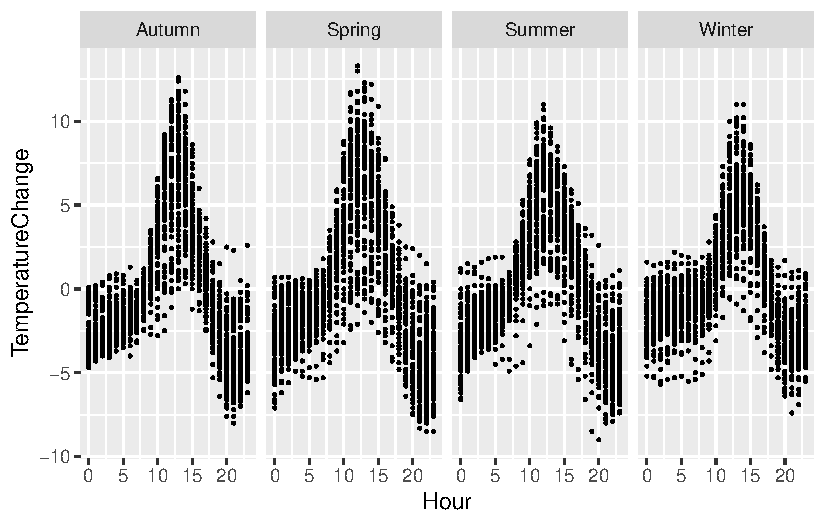
\includegraphics{seoul_files/figure-pdf/unnamed-chunk-3-1.pdf}

According to our model, changes in temperature not only depend on
temperature but also on season. While there are some general linear
trends across some ranges of hours, the non-linearity of the hours in
general with respect to temperature change led us to include indicators
for each hour as specified in Model (1) using Hour 0 (12:00 a.m.) as our
base year.

According to the model diagnostics \protect\hyperlink{a10}{A.1.0}, the
linearity assumption seems to met (see \protect\hyperlink{a11}{A.1} for
added variable plots). Additionally, though there were some points
moving the model away from homoskedasticity the
\(\sqrt{|\text{standardized residuals}|)}\) vs.~Fitted values Plot shows
that homoskedasticity is roughly met. However, the normality assumption
was blatantly violated so we considered adding in interaction terms.

We used elastic net regression to select interaction terms to see if the
influential points (and thus, Normality) could be remedied. We used
elastic net regression over lasso regression due to the potential
colinearity between \(\text{HumidityChange}_{st}\) and other weather
effects.

(The summary output is too long to be included here, see
\protect\hyperlink{a20}{A.2.0} for model output)

However, even with selected interaction terms included, Normality did
not drastically improve (see \protect\hyperlink{a21}{A.2.1} for
QQ-Plot).

We considered transforming the model (\protect\hyperlink{a3}{A.3}) to
better meet Normality and somewhat homoskedasticity. However, due to the
nature of our \(X\) variable matrix--since each independent variable is
a change in a variable, we thus had to shift the entire vector of that
corresponding variable in order to derive optimal transformations.
Hence, interpreting the any transformations we would make would prove
difficult and impractical.

However, with large sample size (\(n=8740\)), Normality could be
appealed to. The residuals do appear to be Normal, though extreme values
cause deviations from Normality at the tails as seen in the QQ-plot. We
considered alternatives to meeting the assumptions such as linear robust
regression to reduce the weights of outliers. One alternative is further
discussed in \protect\hyperlink{a4}{A.4}, where we considered estimating
a model for each season.

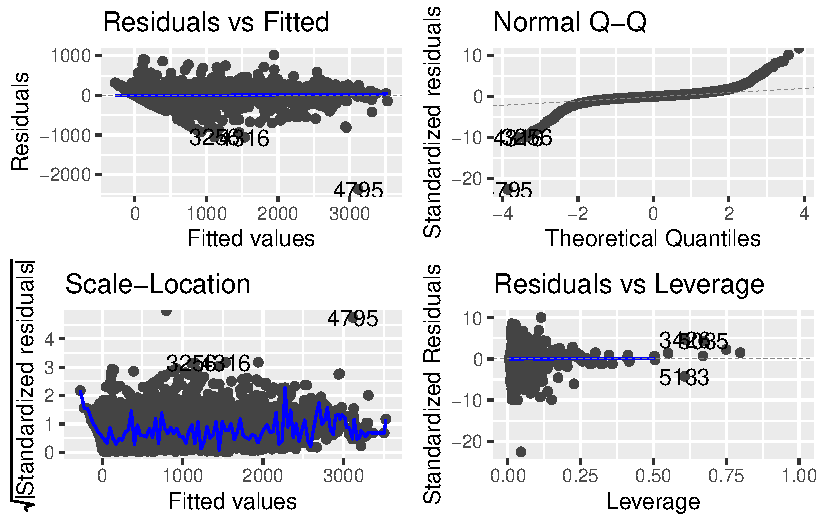
\includegraphics{seoul_files/figure-pdf/unnamed-chunk-6-1.pdf}

Since the histogram of the residuals appears Normal, aside from the
extreme values at the tails, we will appeal to Normality due to the
large sample size.

Additionally, diagnostics (\protect\hyperlink{a21}{A.2.1}) show that
there no undully outliers, and linearity and homoskedasticity are met.

Thus, using our elastic regression results, we will modify Model (1) to
include the following interaction terms. We made sure to include the
lower-order regression coefficients for the coefficients that elastic
net regression left out when elastic net included interaction terms
involving a lower-order term. We are interested in estimating the most
assailant factors (\protect\hyperlink{a5}{A.5}). See
\protect\hyperlink{a6}{A.6} for the full model.

\begin{enumerate}
\def\labelenumi{(\arabic{enumi})}
\setcounter{enumi}{1}
\tightlist
\item
  \(\Delta\text{Temperature}_{st} = ... + \beta_5\Delta\text{SolarRadiation}_{st} + ... + \beta_8\Delta I(\text{Hour}_{t} = 1) + ... + \beta_{30}\Delta I(\text{Hour}_{t} = 23) + ... + \beta_{32}\Delta\text{Humidity}_{st}\text{SolarRadiation}_{st} + ... + \beta_{39}\Delta\text{SolarRadiation}_{st}\text{Rainfall}_{st} + ... + \sum_{n=1}^{23}{\beta_{131+n}\Delta\text{SolarRadiation}_{st}\Delta I(\text{Hour}_t=n)} + ... + \Delta\eta_{st}\)
\end{enumerate}

\(\Delta\eta_{st} \overset{iid}{\sim} N(0, \sigma^2)\)

\begin{center}\rule{0.5\linewidth}{0.5pt}\end{center}

In order to estimate the hourly demand for bike sharing in Seoul.
Similar to our model for temperature, we have unobserved seasonal
effects in \(\epsilon\). However, exploratory data analysis has shown
that current bike demand is not strongly dependent on the bike demand
from \(t-1\). Instead of using a first-difference approach, we will use
a fixed effects models to include the seasonal effects for \(s-1\) (3)
seasons to obtain unbiased estimates. We will use Spring as our base
season.

\begin{Shaded}
\begin{Highlighting}[]
\NormalTok{l }\OtherTok{=} \DecValTok{1}
\NormalTok{alpha }\OtherTok{=} \FloatTok{0.05}
\NormalTok{deltas }\OtherTok{=} \FunctionTok{cov}\NormalTok{(seoul}\SpecialCharTok{$}\NormalTok{RentedBikeCount[(l}\SpecialCharTok{+}\DecValTok{1}\NormalTok{)}\SpecialCharTok{:}\FunctionTok{length}\NormalTok{(seoul}\SpecialCharTok{$}\NormalTok{RentedBikeCount)], }
    \FunctionTok{lag}\NormalTok{(seoul}\SpecialCharTok{$}\NormalTok{RentedBikeCount, }\AttributeTok{n=}\NormalTok{l)[(l}\SpecialCharTok{+}\DecValTok{1}\NormalTok{)}\SpecialCharTok{:}\FunctionTok{length}\NormalTok{(seoul}\SpecialCharTok{$}\NormalTok{RentedBikeCount)])}\SpecialCharTok{/}
\FunctionTok{var}\NormalTok{(seoul}\SpecialCharTok{$}\NormalTok{RentedBikeCount[(l}\SpecialCharTok{+}\DecValTok{1}\NormalTok{)}\SpecialCharTok{:}\FunctionTok{length}\NormalTok{(seoul}\SpecialCharTok{$}\NormalTok{RentedBikeCount)])}
\NormalTok{p.value }\OtherTok{=} \DecValTok{0}

\ControlFlowTok{while}\NormalTok{(p.value }\SpecialCharTok{\textless{}}\NormalTok{ alpha)\{}
\NormalTok{  l }\OtherTok{=}\NormalTok{ l}\SpecialCharTok{+}\DecValTok{1}
  
\NormalTok{  deltas }\OtherTok{=} \FunctionTok{c}\NormalTok{(deltas, }\FunctionTok{cov}\NormalTok{(seoul}\SpecialCharTok{$}\NormalTok{RentedBikeCount[(l}\SpecialCharTok{+}\DecValTok{1}\NormalTok{)}\SpecialCharTok{:}\FunctionTok{length}\NormalTok{(seoul}\SpecialCharTok{$}\NormalTok{RentedBikeCount)], }
    \FunctionTok{lag}\NormalTok{(seoul}\SpecialCharTok{$}\NormalTok{RentedBikeCount, }\AttributeTok{n=}\NormalTok{l)[(l}\SpecialCharTok{+}\DecValTok{1}\NormalTok{)}\SpecialCharTok{:}\FunctionTok{length}\NormalTok{(seoul}\SpecialCharTok{$}\NormalTok{RentedBikeCount)])}\SpecialCharTok{/}
  \FunctionTok{var}\NormalTok{(seoul}\SpecialCharTok{$}\NormalTok{RentedBikeCount[(l}\SpecialCharTok{+}\DecValTok{1}\NormalTok{)}\SpecialCharTok{:}\FunctionTok{length}\NormalTok{(seoul}\SpecialCharTok{$}\NormalTok{RentedBikeCount)]))}
  
\NormalTok{  l.lm }\OtherTok{=} \FunctionTok{lm}\NormalTok{(seoul}\SpecialCharTok{$}\NormalTok{RentedBikeCount[(l}\SpecialCharTok{+}\DecValTok{1}\NormalTok{)}\SpecialCharTok{:}\FunctionTok{length}\NormalTok{(seoul}\SpecialCharTok{$}\NormalTok{RentedBikeCount)] }\SpecialCharTok{\textasciitilde{}} 
       \FunctionTok{lag}\NormalTok{(seoul}\SpecialCharTok{$}\NormalTok{RentedBikeCount, }\AttributeTok{n=}\NormalTok{l)[(l}\SpecialCharTok{+}\DecValTok{1}\NormalTok{)}\SpecialCharTok{:}\FunctionTok{length}\NormalTok{(seoul}\SpecialCharTok{$}\NormalTok{RentedBikeCount)]) }\SpecialCharTok{\%\textgreater{}\%}
    \FunctionTok{summary}\NormalTok{()}
\NormalTok{  p.value }\OtherTok{=}\NormalTok{ l.lm}\SpecialCharTok{$}\NormalTok{coefficients[, }\StringTok{"Pr(\textgreater{}|t|)"}\NormalTok{][}\DecValTok{2}\NormalTok{]}
\NormalTok{\}}

\NormalTok{find\_local\_max }\OtherTok{=} \ControlFlowTok{function}\NormalTok{(v)\{}
  \ControlFlowTok{if}\NormalTok{(v[}\DecValTok{2}\NormalTok{] }\SpecialCharTok{\textless{}=}\NormalTok{ v[}\DecValTok{1}\NormalTok{])\{}
\NormalTok{    maxes }\OtherTok{=}\NormalTok{ v[}\DecValTok{1}\NormalTok{]}
\NormalTok{  \} }\ControlFlowTok{else}\NormalTok{ \{}
\NormalTok{    maxes }\OtherTok{=} \FunctionTok{c}\NormalTok{()}
\NormalTok{  \}}
  
  \ControlFlowTok{for}\NormalTok{(i }\ControlFlowTok{in} \DecValTok{1}\SpecialCharTok{:}\FunctionTok{length}\NormalTok{(v))\{}
    \ControlFlowTok{if}\NormalTok{(i}\DecValTok{{-}1} \SpecialCharTok{\textgreater{}=} \DecValTok{1} \SpecialCharTok{\&\&}\NormalTok{ i}\SpecialCharTok{+}\DecValTok{1} \SpecialCharTok{\textless{}=} \FunctionTok{length}\NormalTok{(v))\{}
      \ControlFlowTok{if}\NormalTok{(v[i}\DecValTok{{-}1}\NormalTok{] }\SpecialCharTok{\textless{}=}\NormalTok{ v[i] }\SpecialCharTok{\&\&} 
\NormalTok{         v[i}\SpecialCharTok{+}\DecValTok{1}\NormalTok{] }\SpecialCharTok{\textless{}=}\NormalTok{ v[i])\{}
\NormalTok{        maxes }\OtherTok{=} \FunctionTok{c}\NormalTok{(maxes, v[i])}
\NormalTok{      \}}
\NormalTok{    \}}
\NormalTok{  \}}
  
  \ControlFlowTok{if}\NormalTok{(v[}\FunctionTok{length}\NormalTok{(v)] }\SpecialCharTok{\textgreater{}=}\NormalTok{ v[(}\FunctionTok{length}\NormalTok{(v)}\SpecialCharTok{{-}}\DecValTok{1}\NormalTok{)])\{}
\NormalTok{    maxes }\OtherTok{=} \FunctionTok{c}\NormalTok{(maxes, v[}\FunctionTok{length}\NormalTok{(v)])}
\NormalTok{  \}}
  
  \FunctionTok{return}\NormalTok{(maxes)}
\NormalTok{\}}

\NormalTok{local.max }\OtherTok{=} \FunctionTok{find\_local\_max}\NormalTok{(deltas)}
\NormalTok{deltas.max }\OtherTok{=} \FunctionTok{which}\NormalTok{(deltas }\SpecialCharTok{\%in\%}\NormalTok{ local.max)}

\FunctionTok{ggplot}\NormalTok{(}\AttributeTok{mapping=}\FunctionTok{aes}\NormalTok{(}\AttributeTok{x=}\DecValTok{1}\SpecialCharTok{:}\NormalTok{l, }\AttributeTok{y=}\NormalTok{deltas))}\SpecialCharTok{+}
  \FunctionTok{geom\_point}\NormalTok{()}\SpecialCharTok{+}
  \FunctionTok{geom\_line}\NormalTok{()}\SpecialCharTok{+}
  \FunctionTok{xlab}\NormalTok{(}\StringTok{"Lags (Hours Ago)"}\NormalTok{)}\SpecialCharTok{+}
  \FunctionTok{ylab}\NormalTok{(}\FunctionTok{expression}\NormalTok{(delta))}\SpecialCharTok{+}
  \FunctionTok{scale\_x\_continuous}\NormalTok{(}\AttributeTok{breaks=}\NormalTok{deltas.max)}
\end{Highlighting}
\end{Shaded}

\begin{figure}[H]

{\centering 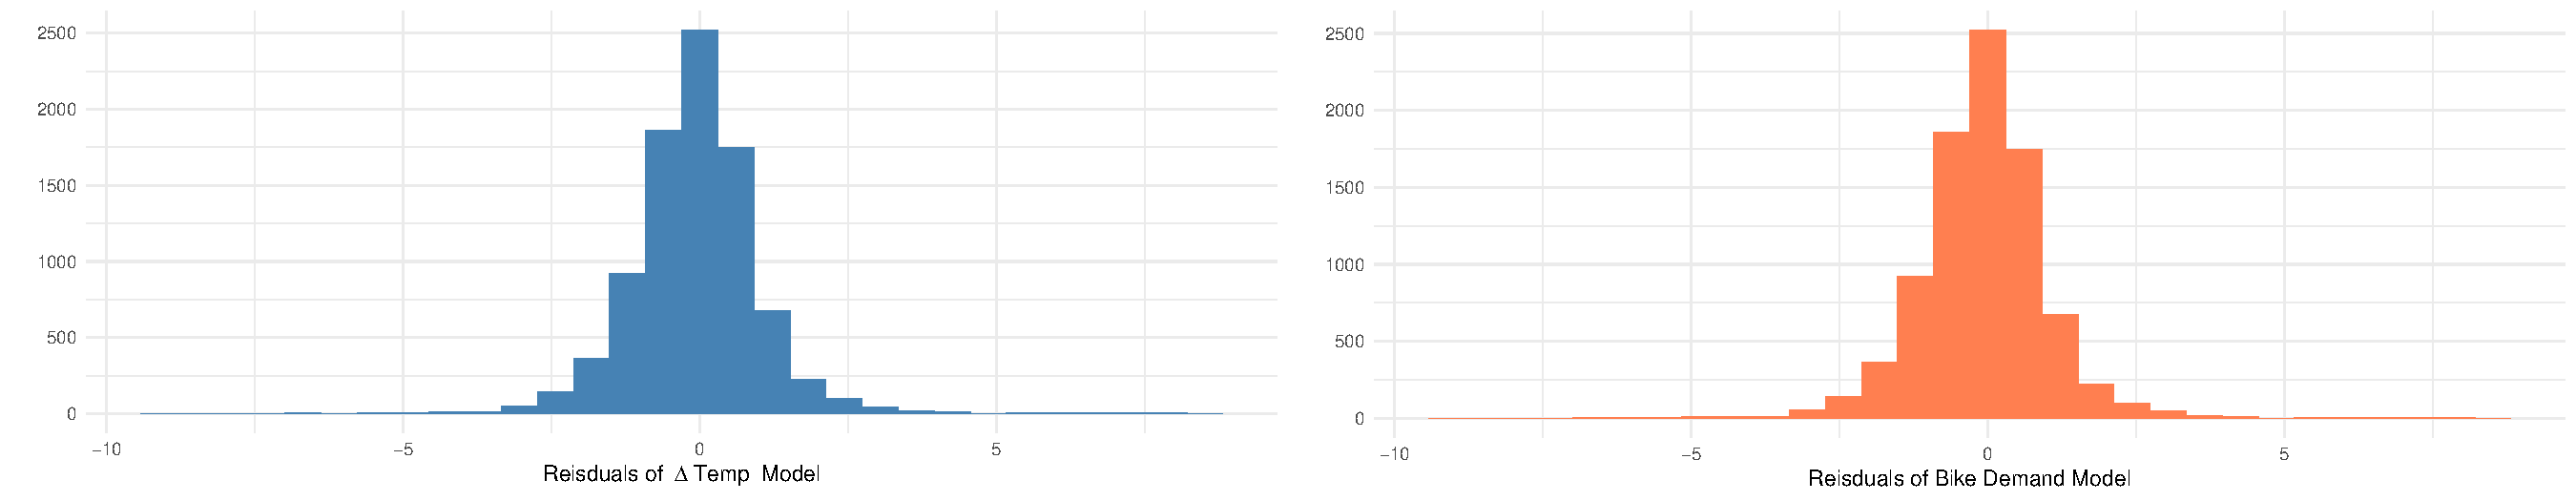
\includegraphics{seoul_files/figure-pdf/unnamed-chunk-7-1.pdf}

}

\end{figure}

We transformed \(\text{RentedBikeCount}_{st}\) with a \(ln\)
transformation. Upon further analysis, we also transformed
\(\text{Visibility}_{st}\) with a \(f(x)=-\sqrt{x}\) transformation. We
also noticed that different levels of \(\text{Humidity}_{st}\) were
affecting \(\text{RentedBikeCount}_{st}\) in a non-linear fashion.
Hence, we created 10 different levels for humidity as dummy variables,
omitting the 0-10\% level as the base level. We also noticed that
extreme levels of \(\text{WindSpeed}_{st}\) were also affecting
\(\text{RentedBikeCount}_{st}\). We created another variable,
\(I(\text{WindSpeed}_{st} > \phi(\text{WindSpeed}_s,0.95))\)

Hence, our basic fixed effects multivariate model for measuring the
demand for rented bikes in Seoul will be interpreted as,

\(ln(\text{RentedBikeCount}_{st}+1) = \beta_0 + \beta_1I(10 \leq Humidity_t < 20) + ... + \beta9I(90 \leq Humidity_t < 100) + \beta_{10}\text{Temperature}_{st} + \beta_{11}\text{WindSpeed}_{st} + \beta_{12}(-\sqrt{\text{Visibility}_{st}}) + \beta_{13}I(\text{ExtremeWind}_{st} = \text{Yes}) + \beta_{14}\text{DewPointTemp}_{st} + \beta_{15}\text{SolarRadiation}_{st} + \beta_{16}\text{Rainfall}_{st} + \beta_{17}\text{Snowfall}_{st} + \beta_{18}I(\text{Day}_t = Holiday) + \beta_{19}I(\text{Hour}_t = 1) + ... + \beta_{41}I(\text{Hour}_t = 23) + \beta_{42}I(\text{Season}_s = Winter) + \beta_{43}I(\text{Season}_s = Summer) + \beta_{44}I(\text{Season}_s = Autumn) + \eta_{st}\)

\hypertarget{appendix}{%
\subsection{APPENDIX}\label{appendix}}

\hypertarget{a0}{%
\paragraph{A.0}\label{a0}}

Selection Process for Optimal Choice of \(k\)

We want \(k\) as small as possible because we want as much data for our
model: Our belief is that short-run fluctuations in temperature can be
determined by other short-run changes in other factors. Hence, the
smaller \(k\) is, the better predictions we can make about the hour
\(t\). If we wanted to parse out a long-run effect, we would aggregate
on a time period and regress over that interval. However, for the
purposes of our research question, we need to be informed the most about
what is happening in the short-run.

Running a \(k\)th difference regression model where
\(\Delta\text{Temperature}_t = \text{Temperature}_t - \text{Temperature}_{t-k}\)
we can find a sufficient \(k\) by regressing
\(\Delta\text{Temperature}_{t-1}\) on
\(\Delta\text{Temperature}_{t-k^*}\), where \(k*\) is the proposed value
of \(k\). We will choose \(k=k^*\) when the regression coefficient
becomes non-significant. This (non-coincidentally) happens as the
regression coefficient approaches 0, or as
\(\Delta\text{Temperature}_t\) becomes less and less dependent of the
\(\Delta\text{Temperature}\) from \(k^*\) hours ago.

The optimal choice of \(k\) will lead us to run a \(k\)th difference
regression model where
\(\Delta\text{Temperature}_t = \text{Temperature}_t - \text{Temperature}_{t-k}\).

Optimal choice of \(k\):

\begin{Shaded}
\begin{Highlighting}[]
\NormalTok{ks }\OtherTok{=} \FunctionTok{c}\NormalTok{()}
\NormalTok{alpha }\OtherTok{=} \FloatTok{0.1}
\ControlFlowTok{for}\NormalTok{(k }\ControlFlowTok{in} \DecValTok{1}\SpecialCharTok{:}\DecValTok{100}\NormalTok{)\{}
\NormalTok{  k.change }\OtherTok{=}\NormalTok{ seoul}\SpecialCharTok{$}\NormalTok{Temperature }\SpecialCharTok{{-}} \FunctionTok{lag}\NormalTok{(seoul}\SpecialCharTok{$}\NormalTok{Temperature, }\AttributeTok{n =} \DecValTok{1}\NormalTok{)}
\NormalTok{  k.lm }\OtherTok{=} \FunctionTok{lm}\NormalTok{(k.change }\SpecialCharTok{\textasciitilde{}} \FunctionTok{lag}\NormalTok{(k.change, }\AttributeTok{n =}\NormalTok{ k))}
\NormalTok{  k.p }\OtherTok{=} \FunctionTok{summary}\NormalTok{(k.lm)}\SpecialCharTok{$}\NormalTok{coefficients[, }\StringTok{"Pr(\textgreater{}|t|)"}\NormalTok{][}\DecValTok{2}\NormalTok{]}
  \ControlFlowTok{if}\NormalTok{(k.p }\SpecialCharTok{\textgreater{}}\NormalTok{ alpha)\{}
\NormalTok{    ks }\OtherTok{=} \FunctionTok{c}\NormalTok{(ks, k)}
\NormalTok{  \}}
\NormalTok{\}}

\NormalTok{ks}
\end{Highlighting}
\end{Shaded}

\begin{verbatim}
[1]  5 19 29 43 53 67 77 91
\end{verbatim}

Hence, we chose \(k\) = 5

\hypertarget{a10}{%
\paragraph{A.1.0}\label{a10}}

Regression output and diagnostics for Model (1)

\begin{Shaded}
\begin{Highlighting}[]
\NormalTok{seoul.lm }\OtherTok{=} \FunctionTok{lm}\NormalTok{(TemperatureChange }\SpecialCharTok{\textasciitilde{}} \DecValTok{0} \SpecialCharTok{+}\NormalTok{ ., }\AttributeTok{data=}\NormalTok{seoul.temp[}\FunctionTok{c}\NormalTok{(seoul.change)])}
\FunctionTok{summary}\NormalTok{(seoul.lm)}
\end{Highlighting}
\end{Shaded}

\begin{verbatim}

Call:
lm(formula = TemperatureChange ~ 0 + ., data = seoul.temp[c(seoul.change)])

Residuals:
    Min      1Q  Median      3Q     Max 
-9.9593 -0.5910  0.0285  0.6114 11.6173 

Coefficients:
                       Estimate Std. Error t value Pr(>|t|)    
HumidityChange       -1.439e-01  1.854e-03 -77.608  < 2e-16 ***
DewPointTempChange    5.144e-01  7.553e-03  68.099  < 2e-16 ***
WindSpeedChange       6.783e-02  1.375e-02   4.932 8.30e-07 ***
VisibilityChange     -3.087e-04  3.525e-05  -8.759  < 2e-16 ***
SolarRadiationChange  1.091e+00  2.495e-02  43.712  < 2e-16 ***
RainfallChange        6.186e-03  8.905e-03   0.695  0.48729    
SnowfallChange        2.268e-01  4.329e-02   5.240 1.65e-07 ***
Hour1Change          -1.645e-01  1.256e-01  -1.310  0.19034    
Hour2Change          -3.219e-01  1.526e-01  -2.110  0.03487 *  
Hour3Change          -4.914e-01  1.499e-01  -3.279  0.00105 ** 
Hour4Change          -6.358e-01  1.156e-01  -5.501 3.89e-08 ***
Hour5Change          -7.538e-01  6.261e-02 -12.040  < 2e-16 ***
Hour6Change          -8.368e-01  1.344e-01  -6.224 5.06e-10 ***
Hour7Change          -9.824e-01  1.546e-01  -6.355 2.19e-10 ***
Hour8Change          -9.756e-01  1.464e-01  -6.662 2.87e-11 ***
Hour9Change          -9.226e-01  1.042e-01  -8.855  < 2e-16 ***
Hour10Change         -6.220e-01  9.017e-02  -6.898 5.64e-12 ***
Hour11Change         -2.461e-01  1.454e-01  -1.693  0.09054 .  
Hour12Change          1.687e-01  1.605e-01   1.051  0.29338    
Hour13Change          5.972e-01  1.478e-01   4.041 5.37e-05 ***
Hour14Change          1.084e+00  9.636e-02  11.245  < 2e-16 ***
Hour15Change          1.463e+00  1.101e-01  13.286  < 2e-16 ***
Hour16Change          1.743e+00  1.501e-01  11.612  < 2e-16 ***
Hour17Change          1.770e+00  1.570e-01  11.274  < 2e-16 ***
Hour18Change          1.627e+00  1.361e-01  11.958  < 2e-16 ***
Hour19Change          1.327e+00  6.489e-02  20.445  < 2e-16 ***
Hour20Change          9.682e-01  1.161e-01   8.341  < 2e-16 ***
Hour21Change          6.576e-01  1.500e-01   4.383 1.19e-05 ***
Hour22Change          3.900e-01  1.526e-01   2.555  0.01063 *  
Hour23Change          1.628e-01  1.257e-01   1.295  0.19535    
---
Signif. codes:  0 '***' 0.001 '**' 0.01 '*' 0.05 '.' 0.1 ' ' 1

Residual standard error: 1.205 on 8710 degrees of freedom
Multiple R-squared:  0.8989,    Adjusted R-squared:  0.8985 
F-statistic:  2581 on 30 and 8710 DF,  p-value: < 2.2e-16
\end{verbatim}

\begin{Shaded}
\begin{Highlighting}[]
\FunctionTok{autoplot}\NormalTok{(seoul.lm)}
\end{Highlighting}
\end{Shaded}

\begin{figure}[H]

{\centering 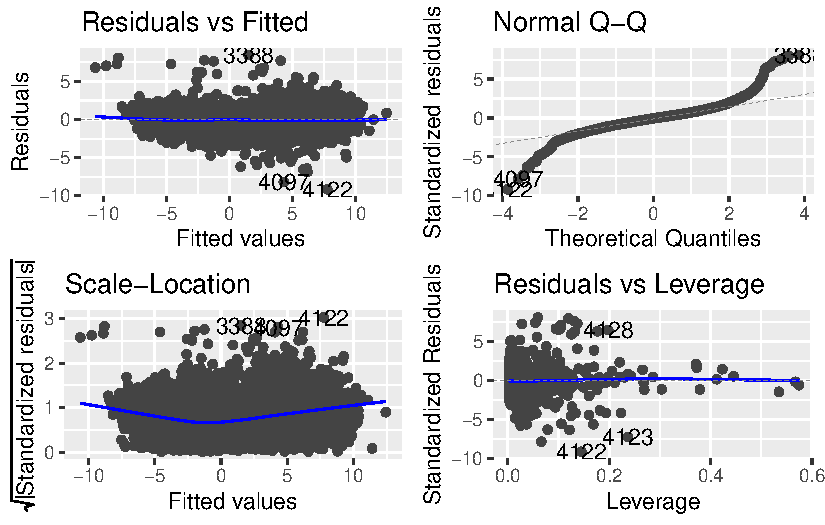
\includegraphics{seoul_files/figure-pdf/unnamed-chunk-9-1.pdf}

}

\end{figure}

\begin{Shaded}
\begin{Highlighting}[]
\FunctionTok{show\_leverage}\NormalTok{(seoul.lm)}
\end{Highlighting}
\end{Shaded}

\begin{figure}[H]

{\centering 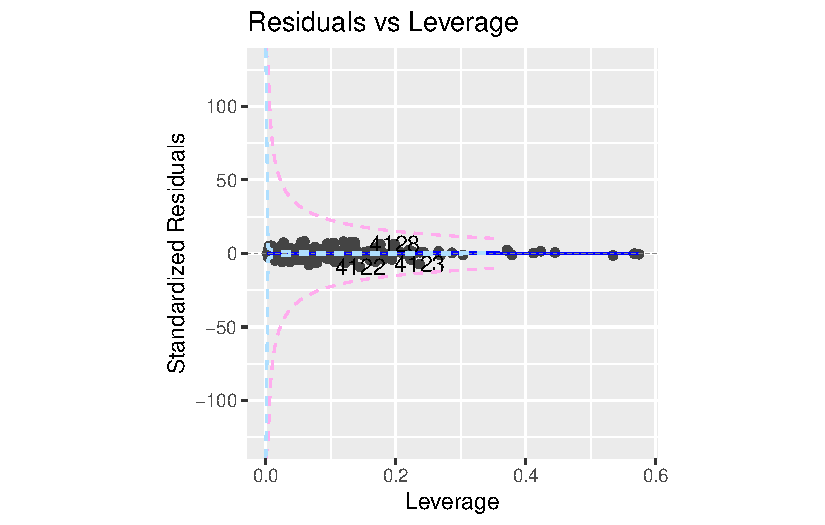
\includegraphics{seoul_files/figure-pdf/unnamed-chunk-9-2.pdf}

}

\end{figure}

\hypertarget{a11}{%
\paragraph{A.1.1}\label{a11}}

Added Variable Plots for Model (1). After considering the influential
points, we determined that the linearity assumption was met.

\begin{Shaded}
\begin{Highlighting}[]
\FunctionTok{avPlots}\NormalTok{(seoul.lm)}
\end{Highlighting}
\end{Shaded}

\begin{figure}[H]

{\centering 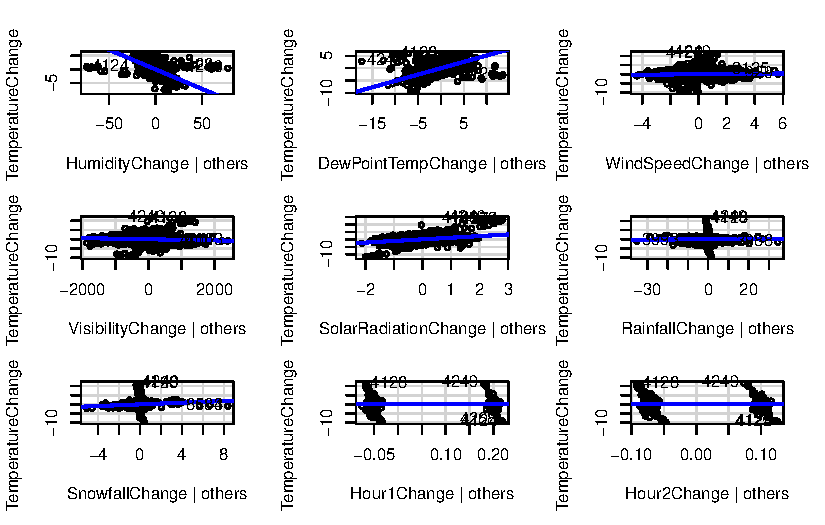
\includegraphics{seoul_files/figure-pdf/unnamed-chunk-10-1.pdf}

}

\end{figure}

\begin{figure}[H]

{\centering 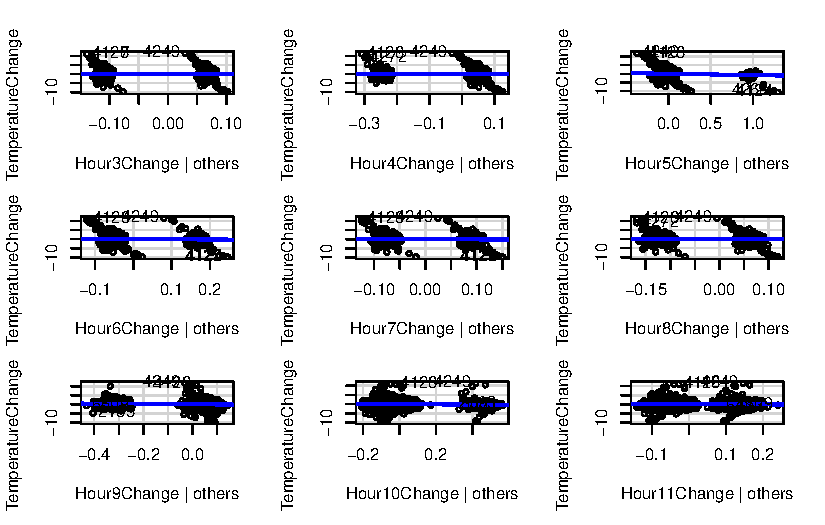
\includegraphics{seoul_files/figure-pdf/unnamed-chunk-10-2.pdf}

}

\end{figure}

\begin{figure}[H]

{\centering 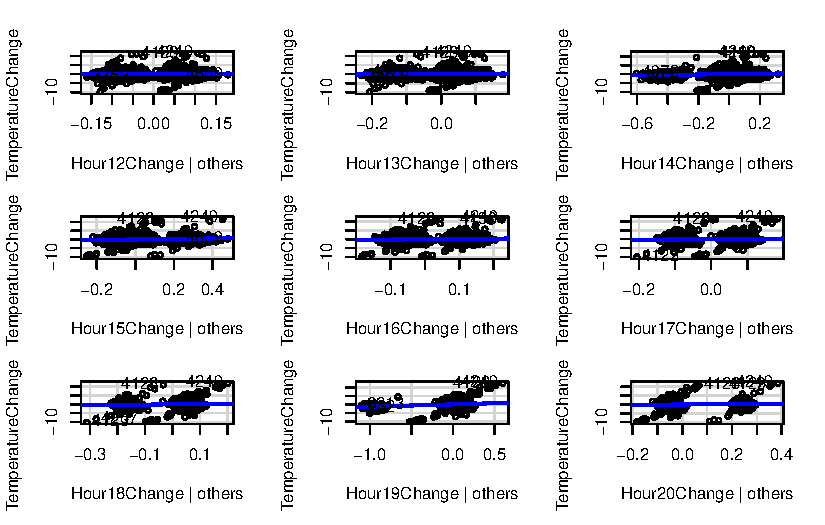
\includegraphics{seoul_files/figure-pdf/unnamed-chunk-10-3.pdf}

}

\end{figure}

\begin{figure}[H]

{\centering 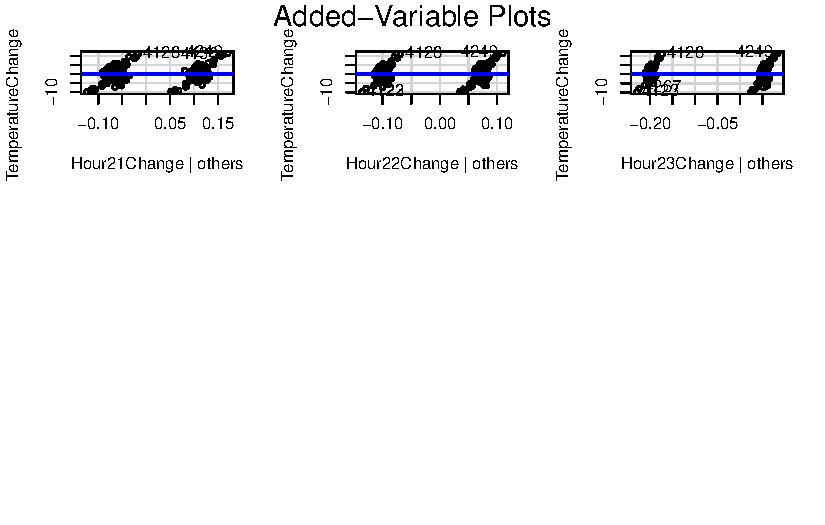
\includegraphics{seoul_files/figure-pdf/unnamed-chunk-10-4.pdf}

}

\end{figure}

\hypertarget{a20}{%
\paragraph{A.2.0}\label{a20}}

Elastic Net Regression on Model (1) w/ interaction terms

\begin{Shaded}
\begin{Highlighting}[]
\FunctionTok{summary}\NormalTok{(seoul.elastic)}
\end{Highlighting}
\end{Shaded}

\begin{verbatim}

Call:
lm(formula = TemperatureChange ~ 0 + ., data = seoul.temp[c("TemperatureChange", 
    elastic.factors)])

Residuals:
    Min      1Q  Median      3Q     Max 
-9.1549 -0.6624 -0.0571  0.4846  8.4839 

Coefficients:
                                       Estimate Std. Error t value Pr(>|t|)    
HumidityChange                       -1.528e-01  1.848e-03 -82.691  < 2e-16 ***
DewPointTempChange                    5.568e-01  7.352e-03  75.726  < 2e-16 ***
WindSpeedChange                       5.138e-02  1.263e-02   4.069 4.77e-05 ***
VisibilityChange                     -3.557e-04  3.229e-05 -11.017  < 2e-16 ***
SolarRadiationChange                  9.373e-01  3.309e-02  28.328  < 2e-16 ***
SnowfallChange                        3.596e-01  4.771e-02   7.537 5.28e-14 ***
Hour3Change                          -3.991e-01  2.482e-01  -1.608 0.107860    
Hour4Change                          -8.994e-01  2.097e-01  -4.289 1.82e-05 ***
Hour5Change                          -8.085e-01  6.284e-02 -12.866  < 2e-16 ***
Hour6Change                          -6.767e-01  2.056e-01  -3.292 0.001000 ** 
Hour7Change                          -4.968e-01  2.449e-01  -2.028 0.042544 *  
Hour8Change                          -7.529e-01  2.453e-01  -3.069 0.002152 ** 
Hour9Change                          -1.062e+00  1.955e-01  -5.434 5.65e-08 ***
Hour10Change                         -6.464e-01  1.261e-01  -5.125 3.04e-07 ***
Hour11Change                         -4.987e-02  2.244e-01  -0.222 0.824140    
Hour13Change                          5.450e-02  2.279e-01   0.239 0.810994    
Hour14Change                          5.829e-01  1.378e-01   4.231 2.35e-05 ***
Hour15Change                          8.100e-01  1.548e-01   5.232 1.71e-07 ***
Hour16Change                          1.251e+00  2.341e-01   5.345 9.25e-08 ***
Hour17Change                          1.062e+00  2.516e-01   4.221 2.46e-05 ***
Hour18Change                          5.973e-01  2.213e-01   2.699 0.006962 ** 
Hour19Change                          6.262e-01  9.809e-02   6.384 1.82e-10 ***
Hour20Change                          7.027e-01  1.920e-01   3.659 0.000255 ***
Hour21Change                          5.671e-01  2.407e-01   2.356 0.018490 *  
HumidityChangeXDewPointTempChange    -1.263e-03  1.952e-04  -6.472 1.02e-10 ***
HumidityChangeXSolarRadiationChange   1.364e-02  1.335e-03  10.221  < 2e-16 ***
HumidityChangeXRainfallChange        -2.264e-03  1.013e-03  -2.236 0.025375 *  
HumidityChangeXSnowfallChange        -3.120e-03  1.492e-03  -2.092 0.036484 *  
DewPointTempChangeXWindSpeedChange    2.054e-02  3.972e-03   5.172 2.37e-07 ***
DewPointTempChangeXRainfallChange    -4.092e-03  5.204e-03  -0.786 0.431623    
WindSpeedChangeXVisibilityChange      7.578e-05  2.644e-05   2.866 0.004161 ** 
WindSpeedChangeXSolarRadiationChange  3.649e-02  1.291e-02   2.826 0.004723 ** 
SolarRadiationChangeXRainfallChange   1.031e-01  2.728e-02   3.779 0.000158 ***
HumidityChangeXHour1Change           -3.931e-02  8.051e-03  -4.883 1.06e-06 ***
HumidityChangeXHour2Change           -3.990e-02  7.915e-03  -5.041 4.72e-07 ***
HumidityChangeXHour4Change            1.307e-02  8.417e-03   1.553 0.120437    
HumidityChangeXHour5Change            5.312e-02  4.720e-03  11.255  < 2e-16 ***
HumidityChangeXHour6Change            4.331e-02  7.050e-03   6.144 8.42e-10 ***
HumidityChangeXHour7Change            2.372e-02  6.993e-03   3.392 0.000697 ***
HumidityChangeXHour8Change            4.330e-02  4.514e-03   9.592  < 2e-16 ***
HumidityChangeXHour9Change            6.672e-02  7.309e-03   9.129  < 2e-16 ***
HumidityChangeXHour10Change           1.105e-01  6.987e-03  15.814  < 2e-16 ***
HumidityChangeXHour11Change           6.769e-02  8.637e-03   7.837 5.16e-15 ***
HumidityChangeXHour12Change           2.448e-02  7.358e-03   3.327 0.000883 ***
HumidityChangeXHour14Change           2.618e-02  8.160e-03   3.209 0.001339 ** 
HumidityChangeXHour15Change           2.447e-02  6.135e-03   3.988 6.72e-05 ***
HumidityChangeXHour16Change           4.964e-03  6.894e-03   0.720 0.471552    
HumidityChangeXHour17Change          -3.544e-03  7.104e-03  -0.499 0.617922    
HumidityChangeXHour19Change           4.920e-02  7.907e-03   6.222 5.14e-10 ***
HumidityChangeXHour22Change          -2.243e-02  5.609e-03  -3.999 6.43e-05 ***
HumidityChangeXHour23Change          -3.629e-02  6.960e-03  -5.213 1.90e-07 ***
DewPointTempChangeXHour1Change        1.850e-01  3.060e-02   6.046 1.54e-09 ***
DewPointTempChangeXHour2Change        1.105e-01  3.087e-02   3.579 0.000347 ***
DewPointTempChangeXHour4Change       -2.039e-03  2.874e-02  -0.071 0.943439    
DewPointTempChangeXHour10Change      -1.671e-01  2.162e-02  -7.730 1.20e-14 ***
DewPointTempChangeXHour11Change      -1.080e-01  2.254e-02  -4.792 1.68e-06 ***
DewPointTempChangeXHour13Change      -1.154e-02  2.071e-02  -0.557 0.577534    
DewPointTempChangeXHour14Change      -9.371e-03  2.477e-02  -0.378 0.705146    
DewPointTempChangeXHour18Change      -6.943e-02  2.201e-02  -3.154 0.001616 ** 
DewPointTempChangeXHour19Change      -1.357e-01  2.768e-02  -4.902 9.66e-07 ***
DewPointTempChangeXHour20Change       5.991e-02  2.411e-02   2.484 0.012999 *  
DewPointTempChangeXHour21Change      -2.943e-02  2.467e-02  -1.193 0.232903    
WindSpeedChangeXHour3Change           7.842e-02  5.043e-02   1.555 0.119957    
WindSpeedChangeXHour4Change           9.360e-02  4.844e-02   1.932 0.053344 .  
WindSpeedChangeXHour5Change           1.530e-01  5.635e-02   2.716 0.006629 ** 
WindSpeedChangeXHour6Change           2.358e-01  5.606e-02   4.205 2.63e-05 ***
WindSpeedChangeXHour10Change         -1.726e-03  6.333e-02  -0.027 0.978263    
WindSpeedChangeXHour11Change          2.175e-02  5.063e-02   0.430 0.667559    
WindSpeedChangeXHour15Change          8.869e-06  5.087e-02   0.000 0.999861    
WindSpeedChangeXHour17Change         -7.514e-02  3.943e-02  -1.906 0.056705 .  
WindSpeedChangeXHour18Change         -4.648e-02  3.901e-02  -1.191 0.233495    
WindSpeedChangeXHour19Change         -6.545e-02  4.145e-02  -1.579 0.114394    
VisibilityChangeXHour1Change         -3.839e-04  1.309e-04  -2.932 0.003375 ** 
VisibilityChangeXHour2Change         -4.989e-04  1.221e-04  -4.087 4.41e-05 ***
VisibilityChangeXHour3Change         -8.249e-05  1.231e-04  -0.670 0.502920    
VisibilityChangeXHour4Change         -2.668e-04  1.553e-04  -1.719 0.085712 .  
VisibilityChangeXHour8Change          3.071e-04  1.207e-04   2.544 0.010968 *  
VisibilityChangeXHour9Change          1.102e-04  1.260e-04   0.875 0.381517    
VisibilityChangeXHour11Change        -1.315e-05  1.318e-04  -0.100 0.920529    
VisibilityChangeXHour16Change         1.461e-04  1.410e-04   1.036 0.300281    
VisibilityChangeXHour17Change         8.039e-05  1.164e-04   0.691 0.489669    
VisibilityChangeXHour19Change         3.042e-04  1.152e-04   2.640 0.008303 ** 
VisibilityChangeXHour20Change        -2.940e-05  1.262e-04  -0.233 0.815784    
VisibilityChangeXHour23Change        -6.304e-04  1.489e-04  -4.235 2.31e-05 ***
SolarRadiationChangeXHour1Change      5.953e+00  1.869e+00   3.185 0.001454 ** 
SolarRadiationChangeXHour2Change      8.983e-01  4.699e-01   1.912 0.055965 .  
SolarRadiationChangeXHour3Change     -5.384e-01  1.635e-01  -3.293 0.000994 ***
SolarRadiationChangeXHour4Change     -9.430e-01  1.202e-01  -7.844 4.89e-15 ***
SolarRadiationChangeXHour5Change     -5.630e-01  1.539e-01  -3.659 0.000255 ***
SolarRadiationChangeXHour7Change     -3.073e-01  1.820e-01  -1.688 0.091360 .  
SolarRadiationChangeXHour10Change     5.051e-01  1.182e-01   4.275 1.93e-05 ***
SolarRadiationChangeXHour11Change     8.079e-01  6.633e-02  12.180  < 2e-16 ***
SolarRadiationChangeXHour12Change     4.593e-01  1.533e-01   2.997 0.002737 ** 
SolarRadiationChangeXHour13Change     3.969e-01  5.668e-02   7.002 2.72e-12 ***
SolarRadiationChangeXHour14Change     1.626e-01  6.009e-02   2.706 0.006816 ** 
SolarRadiationChangeXHour17Change    -2.006e-01  1.111e-01  -1.806 0.071030 .  
SolarRadiationChangeXHour20Change    -1.126e-01  7.830e-02  -1.438 0.150593    
SolarRadiationChangeXHour23Change     5.274e-01  1.593e-01   3.311 0.000934 ***
RainfallChangeXHour9Change           -8.069e-02  4.029e-02  -2.003 0.045217 *  
RainfallChangeXHour10Change          -1.236e-01  4.530e-02  -2.729 0.006358 ** 
RainfallChangeXHour14Change           7.073e-02  5.236e-02   1.351 0.176790    
RainfallChangeXHour20Change           5.533e-02  2.055e-02   2.692 0.007113 ** 
RainfallChangeXHour21Change           3.724e-02  2.211e-02   1.685 0.092120 .  
SnowfallChangeXHour8Change           -1.881e-01  1.467e-01  -1.282 0.199705    
SnowfallChangeXHour9Change           -7.721e-02  1.265e-01  -0.610 0.541755    
SnowfallChangeXHour10Change          -2.216e-01  1.034e-01  -2.142 0.032188 *  
SnowfallChangeXHour19Change           4.066e-01  2.400e-01   1.694 0.090332 .  
Hour1Change                           1.230e-01  2.034e-01   0.605 0.545425    
Hour2Change                           1.433e-02  2.454e-01   0.058 0.953451    
Hour12Change                          1.448e-01  2.506e-01   0.578 0.563341    
Hour22Change                          4.439e-01  2.500e-01   1.775 0.075853 .  
Hour23Change                         -5.081e-02  2.145e-01  -0.237 0.812705    
---
Signif. codes:  0 '***' 0.001 '**' 0.01 '*' 0.05 '.' 0.1 ' ' 1

Residual standard error: 1.08 on 8628 degrees of freedom
Multiple R-squared:  0.9195,    Adjusted R-squared:  0.9185 
F-statistic: 880.1 on 112 and 8628 DF,  p-value: < 2.2e-16
\end{verbatim}

\hypertarget{a21}{%
\paragraph{A.2.1}\label{a21}}

Model diagnostics for elastic net regression on Model (1) w/ interaction
terms

Model assumptions did not drastically improve. QQ-plot indicates that
normality assumption is still violated, and is confirmed by a
Shapiro-Wilk normality test.

\begin{Shaded}
\begin{Highlighting}[]
\FunctionTok{autoplot}\NormalTok{(seoul.elastic)}
\end{Highlighting}
\end{Shaded}

\begin{figure}[H]

{\centering 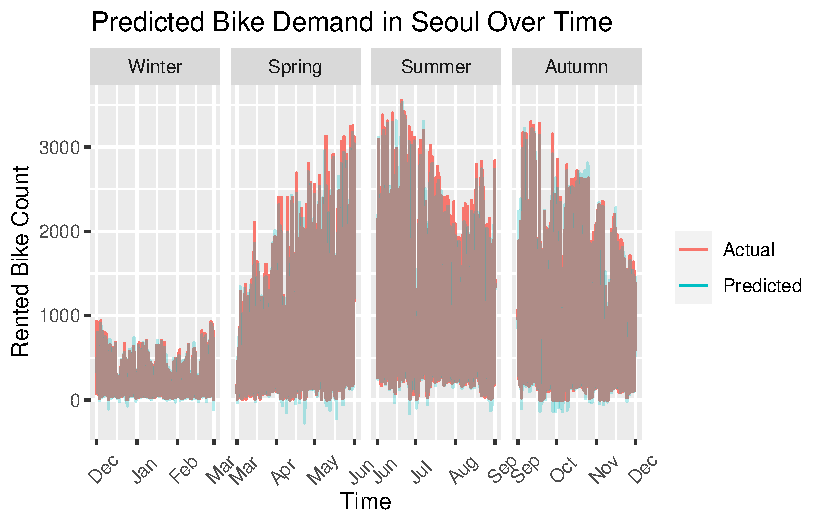
\includegraphics{seoul_files/figure-pdf/unnamed-chunk-12-1.pdf}

}

\end{figure}

\begin{Shaded}
\begin{Highlighting}[]
\FunctionTok{shapiro.test}\NormalTok{(}\FunctionTok{sample}\NormalTok{(seoul.elastic}\SpecialCharTok{$}\NormalTok{residuals, }\DecValTok{5000}\NormalTok{))}
\end{Highlighting}
\end{Shaded}

\begin{verbatim}

    Shapiro-Wilk normality test

data:  sample(seoul.elastic$residuals, 5000)
W = 0.94129, p-value < 2.2e-16
\end{verbatim}

\begin{Shaded}
\begin{Highlighting}[]
\FunctionTok{show\_leverage}\NormalTok{(seoul.elastic)}
\end{Highlighting}
\end{Shaded}

\begin{figure}[H]

{\centering 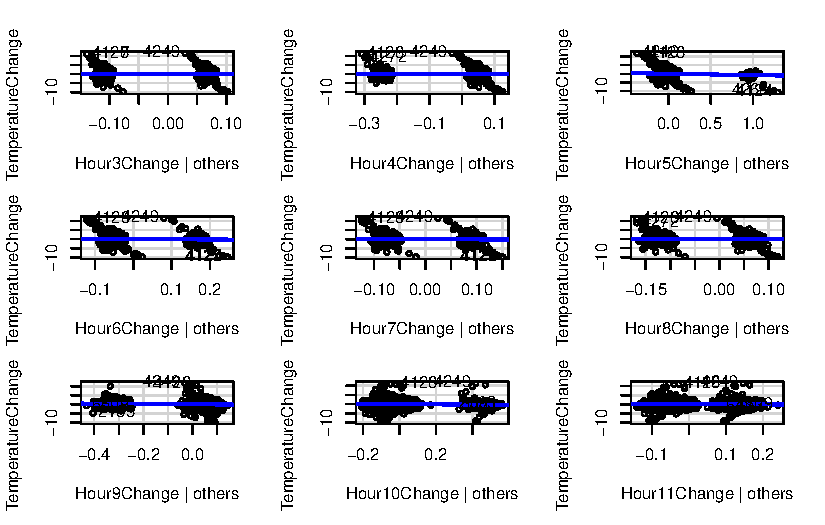
\includegraphics{seoul_files/figure-pdf/unnamed-chunk-12-2.pdf}

}

\end{figure}

\hypertarget{a3}{%
\paragraph{A.3}\label{a3}}

Transformations we considered for Model (1)

\begin{Shaded}
\begin{Highlighting}[]
\NormalTok{factors.transform }\OtherTok{=} \FunctionTok{c}\NormalTok{(}\StringTok{"HumidityChange"}\NormalTok{, }\StringTok{"DewPointTempChange"}\NormalTok{, }
                      \StringTok{"SolarRadiationChange"}\NormalTok{, }\StringTok{"WindSpeedChange"}\NormalTok{)}

\NormalTok{t }\OtherTok{=}\NormalTok{ seoul.temp }\SpecialCharTok{\%\textgreater{}\%} \FunctionTok{mutate}\NormalTok{(}
  \AttributeTok{HumidityChange =}\NormalTok{ HumidityChange }\SpecialCharTok{+} \FunctionTok{abs}\NormalTok{(}\FunctionTok{min}\NormalTok{(HumidityChange)) }\SpecialCharTok{+} \DecValTok{1}\NormalTok{,}
  \AttributeTok{DewPointTempChange =}\NormalTok{ DewPointTempChange }\SpecialCharTok{+} \FunctionTok{abs}\NormalTok{(}\FunctionTok{min}\NormalTok{(DewPointTempChange)) }\SpecialCharTok{+} \DecValTok{1}\NormalTok{,}
  \AttributeTok{SolarRadiationChange =}\NormalTok{ SolarRadiationChange }\SpecialCharTok{+} \FunctionTok{abs}\NormalTok{(}\FunctionTok{min}\NormalTok{(SolarRadiationChange)) }\SpecialCharTok{+} \DecValTok{1}\NormalTok{,}
  \AttributeTok{WindSpeedChange =}\NormalTok{ WindSpeedChange }\SpecialCharTok{+} \FunctionTok{abs}\NormalTok{(}\FunctionTok{min}\NormalTok{(WindSpeedChange)) }\SpecialCharTok{+} \DecValTok{1}
\NormalTok{)}

\ControlFlowTok{for}\NormalTok{(i }\ControlFlowTok{in} \DecValTok{1}\SpecialCharTok{:}\FunctionTok{length}\NormalTok{(factors.transform))\{}
\NormalTok{  factor }\OtherTok{=}\NormalTok{ factors.transform[i]}
  \FunctionTok{invTranPlot}\NormalTok{(}\FunctionTok{formula}\NormalTok{(}\FunctionTok{str\_c}\NormalTok{(}\StringTok{"TemperatureChange \textasciitilde{} "}\NormalTok{, factor)), }\AttributeTok{data=}\NormalTok{t, }
            \AttributeTok{lambda =} \FunctionTok{c}\NormalTok{(}\SpecialCharTok{{-}}\DecValTok{1}\NormalTok{, }\SpecialCharTok{{-}}\FloatTok{0.5}\NormalTok{, }\DecValTok{0}\NormalTok{, }\FloatTok{0.5}\NormalTok{, }\DecValTok{1}\NormalTok{, }\DecValTok{2}\NormalTok{), }\AttributeTok{optimal=}\NormalTok{T)}
\NormalTok{\}}
\end{Highlighting}
\end{Shaded}

\begin{figure}[H]

{\centering 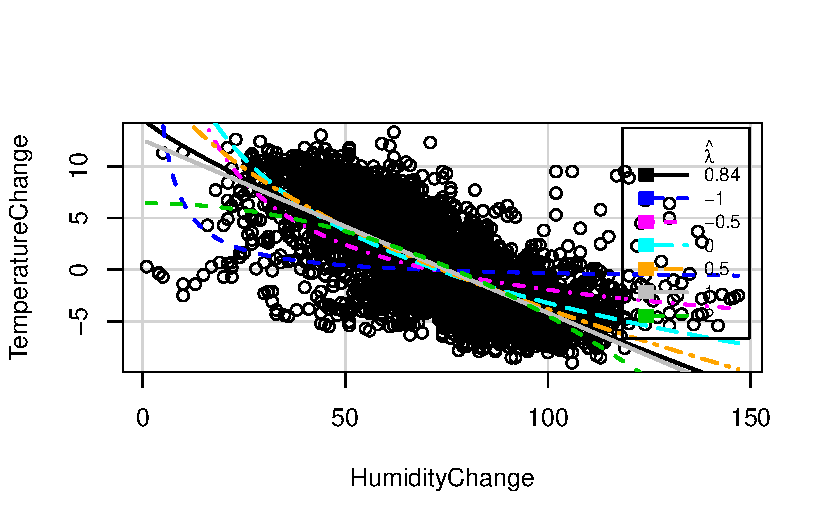
\includegraphics{seoul_files/figure-pdf/unnamed-chunk-13-1.pdf}

}

\end{figure}

\begin{figure}[H]

{\centering 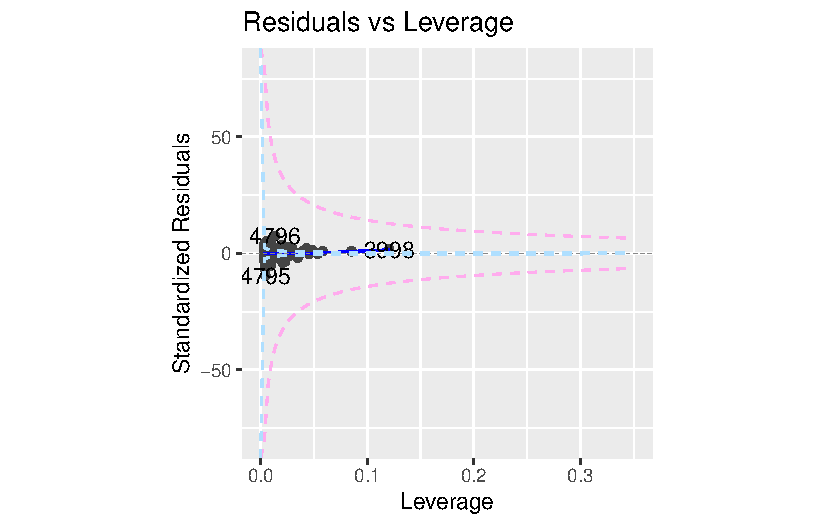
\includegraphics{seoul_files/figure-pdf/unnamed-chunk-13-2.pdf}

}

\end{figure}

\begin{figure}[H]

{\centering 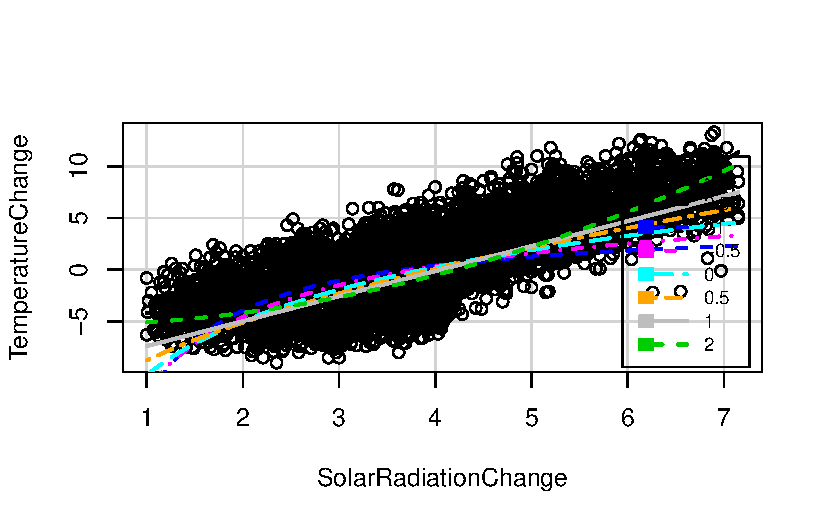
\includegraphics{seoul_files/figure-pdf/unnamed-chunk-13-3.pdf}

}

\end{figure}

\begin{figure}[H]

{\centering 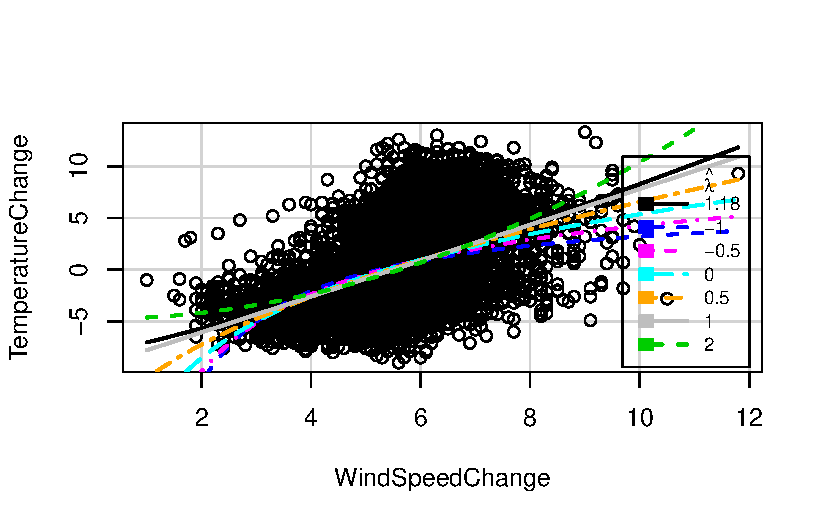
\includegraphics{seoul_files/figure-pdf/unnamed-chunk-13-4.pdf}

}

\end{figure}

\hypertarget{a4}{%
\paragraph{A.4}\label{a4}}

An alternative solution to meeting the assumptions for Model (1). In
theory,

\(\text{Var}(\eta_{st}|s) = \sigma^2 \quad \forall s \in \text{Seasons}\)

However, if it's the case that

\(\exists \text{ at least one } s \text{ s.t. } \text{Var}(\eta_{st}|s) \neq \sigma^2\)

Then, we could use 4 separate models for each season to completely
eliminate \(s\) out of the general \(\eta_{st}\). Hence, each season
will have its own population variance for \(\eta_t\).

\begin{Shaded}
\begin{Highlighting}[]
\NormalTok{create\_season\_models }\OtherTok{=} \ControlFlowTok{function}\NormalTok{(factors, response, }\AttributeTok{base=}\NormalTok{F)\{}
\NormalTok{  factors }\OtherTok{=} \FunctionTok{setdiff}\NormalTok{(factors, response)}
  \ControlFlowTok{if}\NormalTok{(base }\SpecialCharTok{==}\NormalTok{ T)\{}
\NormalTok{    f }\OtherTok{=} \DecValTok{0}
\NormalTok{  \} }\ControlFlowTok{else}\NormalTok{ \{}
\NormalTok{    f }\OtherTok{=} \FunctionTok{paste}\NormalTok{(}\FunctionTok{c}\NormalTok{(}\DecValTok{0}\NormalTok{, factors), }\AttributeTok{collapse =} \StringTok{" + "}\NormalTok{)}
\NormalTok{  \}}

\NormalTok{  models }\OtherTok{\textless{}{-}} \FunctionTok{map}\NormalTok{(}\FunctionTok{unique}\NormalTok{(seoul}\SpecialCharTok{$}\NormalTok{Seasons), }\ControlFlowTok{function}\NormalTok{(x)\{}
    \FunctionTok{lm}\NormalTok{(}\FunctionTok{formula}\NormalTok{(}\FunctionTok{paste}\NormalTok{(response, }\StringTok{"\textasciitilde{}"}\NormalTok{, f)),}
       \AttributeTok{data =}\NormalTok{ seoul[seoul}\SpecialCharTok{$}\NormalTok{Seasons }\SpecialCharTok{==}\NormalTok{ x,] }\SpecialCharTok{\%\textgreater{}\%}
         \FunctionTok{select}\NormalTok{(}\FunctionTok{all\_of}\NormalTok{(}\FunctionTok{c}\NormalTok{(factors, response))))}
\NormalTok{  \})}

  \FunctionTok{names}\NormalTok{(models) }\OtherTok{\textless{}{-}} \FunctionTok{str\_c}\NormalTok{(}\StringTok{"seoul.lm."}\NormalTok{, }\FunctionTok{unique}\NormalTok{(seoul}\SpecialCharTok{$}\NormalTok{Seasons))}
  \FunctionTok{return}\NormalTok{(models)}
\NormalTok{\}}

\NormalTok{models.lm }\OtherTok{=} \FunctionTok{create\_season\_models}\NormalTok{(seoul.change, }\StringTok{"TemperatureChange"}\NormalTok{)}

\NormalTok{create\_elastic }\OtherTok{=} \ControlFlowTok{function}\NormalTok{()\{}
\NormalTok{  models }\OtherTok{=} \FunctionTok{list}\NormalTok{()}
\NormalTok{  seasons }\OtherTok{=}\NormalTok{ seoul}\SpecialCharTok{$}\NormalTok{Seasons }\SpecialCharTok{\%\textgreater{}\%} \FunctionTok{unique}\NormalTok{()}
  \ControlFlowTok{for}\NormalTok{(s }\ControlFlowTok{in}\NormalTok{ seasons)\{}
    \CommentTok{\#print(s)}
\NormalTok{    seoul.subset }\OtherTok{=}\NormalTok{ seoul.temp }\SpecialCharTok{\%\textgreater{}\%} \FunctionTok{filter}\NormalTok{(Seasons }\SpecialCharTok{==}\NormalTok{ s)}
\NormalTok{    seoul.x }\OtherTok{=} \FunctionTok{as.matrix}\NormalTok{(seoul.subset[model.factors])}
\NormalTok{    seoul.y }\OtherTok{=} \FunctionTok{as.matrix}\NormalTok{(seoul.subset[}\StringTok{"TemperatureChange"}\NormalTok{])}

\NormalTok{    elastic\_cv }\OtherTok{\textless{}{-}} \FunctionTok{cv.glmnet}\NormalTok{(}\AttributeTok{x =}\NormalTok{ seoul.x,}
                          \AttributeTok{y =}\NormalTok{ seoul.y,}
                          \AttributeTok{type.measure =} \StringTok{"mse"}\NormalTok{,}
                          \AttributeTok{alpha =} \FloatTok{0.5}\NormalTok{)}

\NormalTok{    d }\OtherTok{=} \FunctionTok{coef}\NormalTok{(elastic\_cv, }\AttributeTok{s =} \StringTok{"lambda.1se"}\NormalTok{)[}\DecValTok{2}\SpecialCharTok{:}\NormalTok{(}\FunctionTok{length}\NormalTok{(model.factors)}\SpecialCharTok{{-}}\DecValTok{1}\NormalTok{)]}
\NormalTok{    elastic.factors }\OtherTok{=}\NormalTok{ model.factors[}\FunctionTok{which}\NormalTok{(d }\SpecialCharTok{!=} \DecValTok{0}\NormalTok{)]}
\NormalTok{    models[[}\FunctionTok{str\_c}\NormalTok{(}\StringTok{"seoul.lasso."}\NormalTok{,s)]] }\OtherTok{=} \FunctionTok{lm}\NormalTok{(TemperatureChange }\SpecialCharTok{\textasciitilde{}} \DecValTok{0} \SpecialCharTok{+}\NormalTok{ .,}
\NormalTok{                                           seoul.subset[}\FunctionTok{c}\NormalTok{(}\StringTok{"TemperatureChange"}\NormalTok{,}
\NormalTok{                                           elastic.factors)])}
\NormalTok{  \}}
  \FunctionTok{return}\NormalTok{(models)}
\NormalTok{\}}
\NormalTok{seoul.elastic.models }\OtherTok{=} \FunctionTok{create\_elastic}\NormalTok{()}
\ControlFlowTok{for}\NormalTok{(model }\ControlFlowTok{in}\NormalTok{ seoul.elastic.models)\{}
  \FunctionTok{print}\NormalTok{(}\FunctionTok{summary}\NormalTok{(model))}
  \FunctionTok{print}\NormalTok{(}\FunctionTok{autoplot}\NormalTok{(model))}
\NormalTok{\}}
\end{Highlighting}
\end{Shaded}

\begin{verbatim}

Call:
lm(formula = TemperatureChange ~ 0 + ., data = seoul.subset[c("TemperatureChange", 
    elastic.factors)])

Residuals:
    Min      1Q  Median      3Q     Max 
-3.5457 -0.4913 -0.0279  0.4156  3.8114 

Coefficients:
                                          Estimate Std. Error t value Pr(>|t|)
HumidityChange                          -1.843e-01  3.750e-03 -49.147  < 2e-16
DewPointTempChange                       7.030e-01  1.244e-02  56.511  < 2e-16
WindSpeedChange                          2.830e-02  1.926e-02   1.469 0.141899
VisibilityChange                        -6.260e-04  6.636e-05  -9.433  < 2e-16
SolarRadiationChange                     9.544e-01  7.420e-02  12.862  < 2e-16
SnowfallChange                           3.881e-01  5.566e-02   6.972 4.18e-12
Hour3Change                             -2.995e-01  9.120e-02  -3.284 0.001039
Hour4Change                             -2.517e-01  9.037e-02  -2.785 0.005394
Hour5Change                             -2.729e-01  8.848e-02  -3.084 0.002070
Hour6Change                             -2.575e-01  8.660e-02  -2.974 0.002977
Hour7Change                             -3.413e-01  8.524e-02  -4.005 6.43e-05
Hour8Change                             -5.646e-01  1.234e-01  -4.576 5.01e-06
Hour9Change                             -3.511e-01  1.357e-01  -2.588 0.009724
Hour10Change                            -3.569e-01  1.255e-01  -2.844 0.004492
Hour13Change                             2.447e-01  1.756e-01   1.393 0.163702
Hour14Change                             8.292e-01  1.427e-01   5.811 7.18e-09
Hour15Change                             1.371e+00  1.375e-01   9.975  < 2e-16
Hour16Change                             1.377e+00  1.093e-01  12.601  < 2e-16
Hour17Change                             4.778e-01  1.203e-01   3.971 7.40e-05
Hour18Change                             5.619e-01  1.101e-01   5.105 3.60e-07
Hour19Change                             7.120e-01  9.360e-02   7.607 4.21e-14
Hour20Change                             6.177e-01  9.103e-02   6.785 1.50e-11
Hour21Change                             5.631e-01  8.544e-02   6.591 5.52e-11
HumidityChangeXDewPointTempChange       -1.070e-03  2.607e-04  -4.105 4.20e-05
DewPointTempChangeXWindSpeedChange       6.293e-03  4.403e-03   1.429 0.153092
DewPointTempChangeXSolarRadiationChange  5.476e-02  9.018e-03   6.073 1.49e-09
DewPointTempChangeXSnowfallChange        5.262e-03  1.374e-02   0.383 0.701847
SolarRadiationChangeXSnowfallChange      3.776e-01  8.368e-02   4.513 6.76e-06
HumidityChangeXHour6Change              -3.521e-03  9.654e-03  -0.365 0.715354
HumidityChangeXHour7Change               2.054e-02  5.861e-03   3.504 0.000468
HumidityChangeXHour8Change               2.520e-02  5.646e-03   4.463 8.49e-06
HumidityChangeXHour9Change               1.765e-02  6.530e-03   2.702 0.006939
HumidityChangeXHour14Change             -8.333e-03  5.504e-03  -1.514 0.130148
HumidityChangeXHour15Change             -1.277e-02  4.914e-03  -2.599 0.009411
HumidityChangeXHour16Change             -2.277e-02  5.891e-03  -3.866 0.000114
DewPointTempChangeXHour5Change           7.101e-02  2.506e-02   2.833 0.004650
DewPointTempChangeXHour6Change           1.057e-01  3.715e-02   2.845 0.004490
DewPointTempChangeXHour21Change         -6.507e-02  2.260e-02  -2.880 0.004023
DewPointTempChangeXHour22Change         -3.310e-02  2.235e-02  -1.481 0.138817
DewPointTempChangeXHour23Change         -4.236e-02  2.355e-02  -1.798 0.072263
WindSpeedChangeXHour1Change              1.243e-01  6.636e-02   1.873 0.061160
WindSpeedChangeXHour10Change            -9.483e-02  6.453e-02  -1.470 0.141832
WindSpeedChangeXHour18Change            -9.884e-03  7.284e-02  -0.136 0.892075
WindSpeedChangeXHour19Change            -9.688e-02  5.788e-02  -1.674 0.094310
WindSpeedChangeXHour23Change             7.615e-02  8.353e-02   0.912 0.362106
VisibilityChangeXHour10Change           -7.377e-04  1.966e-04  -3.753 0.000180
VisibilityChangeXHour11Change           -5.866e-04  2.012e-04  -2.916 0.003583
SolarRadiationChangeXHour8Change         2.323e-01  2.664e-01   0.872 0.383376
SolarRadiationChangeXHour9Change        -5.184e-01  1.731e-01  -2.995 0.002781
SolarRadiationChangeXHour11Change        1.030e-01  1.563e-01   0.659 0.509869
SolarRadiationChangeXHour12Change        2.320e-01  1.466e-01   1.583 0.113605
SolarRadiationChangeXHour13Change        4.131e-01  1.551e-01   2.663 0.007793
SolarRadiationChangeXHour16Change       -7.562e-01  1.873e-01  -4.038 5.59e-05
SolarRadiationChangeXHour17Change       -7.809e-01  2.498e-01  -3.126 0.001796
SolarRadiationChangeXHour22Change        1.025e+00  3.840e-01   2.669 0.007657
SolarRadiationChangeXHour23Change        5.384e+00  1.109e+00   4.854 1.30e-06
RainfallChangeXHour10Change              3.478e-01  1.575e-01   2.208 0.027335
RainfallChangeXHour14Change              3.815e-01  1.233e-01   3.095 0.001997
SnowfallChangeXHour16Change             -9.989e-02  1.305e-01  -0.766 0.443991
                                           
HumidityChange                          ***
DewPointTempChange                      ***
WindSpeedChange                            
VisibilityChange                        ***
SolarRadiationChange                    ***
SnowfallChange                          ***
Hour3Change                             ** 
Hour4Change                             ** 
Hour5Change                             ** 
Hour6Change                             ** 
Hour7Change                             ***
Hour8Change                             ***
Hour9Change                             ** 
Hour10Change                            ** 
Hour13Change                               
Hour14Change                            ***
Hour15Change                            ***
Hour16Change                            ***
Hour17Change                            ***
Hour18Change                            ***
Hour19Change                            ***
Hour20Change                            ***
Hour21Change                            ***
HumidityChangeXDewPointTempChange       ***
DewPointTempChangeXWindSpeedChange         
DewPointTempChangeXSolarRadiationChange ***
DewPointTempChangeXSnowfallChange          
SolarRadiationChangeXSnowfallChange     ***
HumidityChangeXHour6Change                 
HumidityChangeXHour7Change              ***
HumidityChangeXHour8Change              ***
HumidityChangeXHour9Change              ** 
HumidityChangeXHour14Change                
HumidityChangeXHour15Change             ** 
HumidityChangeXHour16Change             ***
DewPointTempChangeXHour5Change          ** 
DewPointTempChangeXHour6Change          ** 
DewPointTempChangeXHour21Change         ** 
DewPointTempChangeXHour22Change            
DewPointTempChangeXHour23Change         .  
WindSpeedChangeXHour1Change             .  
WindSpeedChangeXHour10Change               
WindSpeedChangeXHour18Change               
WindSpeedChangeXHour19Change            .  
WindSpeedChangeXHour23Change               
VisibilityChangeXHour10Change           ***
VisibilityChangeXHour11Change           ** 
SolarRadiationChangeXHour8Change           
SolarRadiationChangeXHour9Change        ** 
SolarRadiationChangeXHour11Change          
SolarRadiationChangeXHour12Change          
SolarRadiationChangeXHour13Change       ** 
SolarRadiationChangeXHour16Change       ***
SolarRadiationChangeXHour17Change       ** 
SolarRadiationChangeXHour22Change       ** 
SolarRadiationChangeXHour23Change       ***
RainfallChangeXHour10Change             *  
RainfallChangeXHour14Change             ** 
SnowfallChangeXHour16Change                
---
Signif. codes:  0 '***' 0.001 '**' 0.01 '*' 0.05 '.' 0.1 ' ' 1

Residual standard error: 0.8675 on 2096 degrees of freedom
Multiple R-squared:  0.9291,    Adjusted R-squared:  0.9271 
F-statistic: 465.4 on 59 and 2096 DF,  p-value: < 2.2e-16
\end{verbatim}

\begin{figure}[H]

{\centering 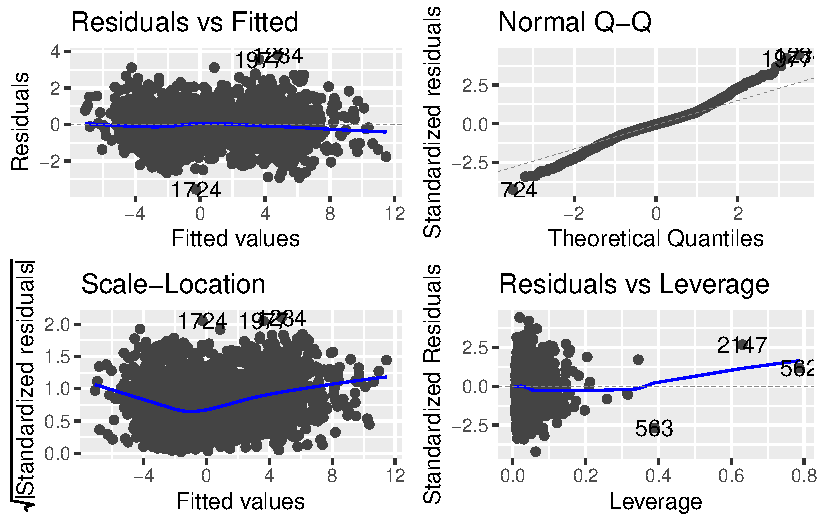
\includegraphics{seoul_files/figure-pdf/unnamed-chunk-14-1.pdf}

}

\end{figure}

\begin{verbatim}

Call:
lm(formula = TemperatureChange ~ 0 + ., data = seoul.subset[c("TemperatureChange", 
    elastic.factors)])

Residuals:
    Min      1Q  Median      3Q     Max 
-6.4208 -0.8507 -0.0578  0.7001  6.3699 

Coefficients:
                                       Estimate Std. Error t value Pr(>|t|)    
HumidityChange                       -9.606e-02  3.395e-03 -28.297  < 2e-16 ***
DewPointTempChange                    3.512e-01  1.404e-02  25.014  < 2e-16 ***
WindSpeedChange                       9.876e-02  3.085e-02   3.201 0.001388 ** 
SolarRadiationChange                  1.421e+00  8.005e-02  17.750  < 2e-16 ***
Hour3Change                          -1.332e+00  1.367e-01  -9.747  < 2e-16 ***
Hour4Change                          -1.275e+00  1.374e-01  -9.283  < 2e-16 ***
Hour5Change                          -1.206e+00  1.319e-01  -9.141  < 2e-16 ***
Hour6Change                          -8.049e-01  1.428e-01  -5.636 1.98e-08 ***
Hour7Change                          -3.888e-01  1.621e-01  -2.399 0.016529 *  
Hour8Change                          -1.409e+00  1.766e-01  -7.978 2.40e-15 ***
Hour9Change                          -1.363e+00  2.465e-01  -5.528 3.64e-08 ***
Hour10Change                         -1.145e+00  2.381e-01  -4.809 1.62e-06 ***
Hour11Change                         -1.046e-01  2.678e-01  -0.391 0.696128    
Hour14Change                          5.763e-01  2.433e-01   2.368 0.017954 *  
Hour15Change                          5.829e-01  2.226e-01   2.618 0.008904 ** 
Hour16Change                          1.676e+00  2.212e-01   7.579 5.15e-14 ***
Hour17Change                          6.493e-01  1.962e-01   3.309 0.000953 ***
Hour18Change                          4.187e-01  2.065e-01   2.027 0.042764 *  
Hour19Change                          1.212e+00  1.913e-01   6.337 2.85e-10 ***
Hour20Change                          9.725e-01  1.543e-01   6.302 3.56e-10 ***
Hour21Change                          1.072e+00  1.458e-01   7.350 2.82e-13 ***
HumidityChangeXDewPointTempChange    -1.618e-03  4.450e-04  -3.637 0.000282 ***
HumidityChangeXSolarRadiationChange   1.649e-02  2.345e-03   7.031 2.74e-12 ***
HumidityChangeXRainfallChange        -1.037e-02  2.768e-03  -3.747 0.000183 ***
DewPointTempChangeXWindSpeedChange   -2.497e-05  7.933e-03  -0.003 0.997489    
DewPointTempChangeXRainfallChange    -3.093e-02  1.258e-02  -2.458 0.014058 *  
WindSpeedChangeXSolarRadiationChange  5.258e-02  2.754e-02   1.909 0.056377 .  
SolarRadiationChangeXRainfallChange   9.620e-02  7.144e-02   1.347 0.178283    
HumidityChangeXHour1Change           -4.008e-02  7.963e-03  -5.032 5.25e-07 ***
HumidityChangeXHour2Change           -3.853e-02  8.820e-03  -4.369 1.31e-05 ***
HumidityChangeXHour5Change            4.327e-02  7.364e-03   5.875 4.89e-09 ***
HumidityChangeXHour8Change            2.569e-02  8.173e-03   3.144 0.001692 ** 
HumidityChangeXHour9Change            3.942e-02  7.417e-03   5.314 1.18e-07 ***
HumidityChangeXHour10Change           8.312e-02  9.686e-03   8.582  < 2e-16 ***
HumidityChangeXHour11Change           5.160e-02  1.069e-02   4.827 1.48e-06 ***
HumidityChangeXHour12Change           1.903e-02  7.992e-03   2.382 0.017325 *  
HumidityChangeXHour16Change          -1.401e-02  9.276e-03  -1.510 0.131200    
HumidityChangeXHour19Change           2.441e-02  9.028e-03   2.704 0.006915 ** 
HumidityChangeXHour22Change          -2.338e-02  8.299e-03  -2.817 0.004899 ** 
HumidityChangeXHour23Change          -3.020e-02  7.528e-03  -4.011 6.25e-05 ***
DewPointTempChangeXHour10Change      -2.113e-01  4.152e-02  -5.089 3.91e-07 ***
DewPointTempChangeXHour11Change      -1.859e-01  4.528e-02  -4.106 4.18e-05 ***
DewPointTempChangeXHour13Change      -5.650e-03  3.242e-02  -0.174 0.861664    
DewPointTempChangeXHour14Change       9.114e-02  3.478e-02   2.621 0.008837 ** 
WindSpeedChangeXHour11Change         -2.031e-01  1.336e-01  -1.520 0.128692    
WindSpeedChangeXHour14Change         -6.747e-02  1.188e-01  -0.568 0.570106    
WindSpeedChangeXHour15Change         -3.019e-03  9.662e-02  -0.031 0.975075    
WindSpeedChangeXHour16Change         -1.243e-01  1.104e-01  -1.126 0.260421    
WindSpeedChangeXHour19Change         -2.895e-01  1.142e-01  -2.535 0.011329 *  
VisibilityChangeXHour2Change         -7.938e-04  2.510e-04  -3.163 0.001584 ** 
VisibilityChangeXHour17Change         4.847e-04  2.076e-04   2.335 0.019648 *  
SolarRadiationChangeXHour1Change      1.694e+01  6.179e+00   2.741 0.006169 ** 
SolarRadiationChangeXHour2Change      2.532e+00  9.657e-01   2.622 0.008803 ** 
SolarRadiationChangeXHour4Change     -1.119e+00  2.459e-01  -4.550 5.67e-06 ***
SolarRadiationChangeXHour5Change     -1.118e+00  1.752e-01  -6.379 2.17e-10 ***
SolarRadiationChangeXHour6Change     -4.865e-01  3.472e-01  -1.401 0.161311    
SolarRadiationChangeXHour7Change     -1.887e-01  3.144e-01  -0.600 0.548467    
SolarRadiationChangeXHour11Change     8.345e-01  2.652e-01   3.146 0.001676 ** 
SolarRadiationChangeXHour12Change     1.102e+00  2.429e-01   4.536 6.06e-06 ***
SolarRadiationChangeXHour13Change     4.572e-01  1.778e-01   2.572 0.010185 *  
SolarRadiationChangeXHour14Change     2.408e-01  1.115e-01   2.160 0.030858 *  
SolarRadiationChangeXHour17Change    -3.973e-01  2.240e-01  -1.773 0.076334 .  
SolarRadiationChangeXHour18Change    -5.142e-01  2.619e-01  -1.963 0.049729 *  
SolarRadiationChangeXHour23Change     1.088e+00  4.082e-01   2.666 0.007735 ** 
RainfallChangeXHour11Change           1.603e-01  1.118e-01   1.434 0.151658    
RainfallChangeXHour14Change           1.326e-01  6.778e-02   1.957 0.050479 .  
RainfallChangeXHour15Change           2.272e-01  1.032e-01   2.202 0.027790 *  
RainfallChangeXHour22Change          -1.941e-01  1.165e-01  -1.666 0.095887 .  
---
Signif. codes:  0 '***' 0.001 '**' 0.01 '*' 0.05 '.' 0.1 ' ' 1

Residual standard error: 1.305 on 2135 degrees of freedom
Multiple R-squared:  0.9059,    Adjusted R-squared:  0.9029 
F-statistic: 302.4 on 68 and 2135 DF,  p-value: < 2.2e-16
\end{verbatim}

\begin{figure}[H]

{\centering 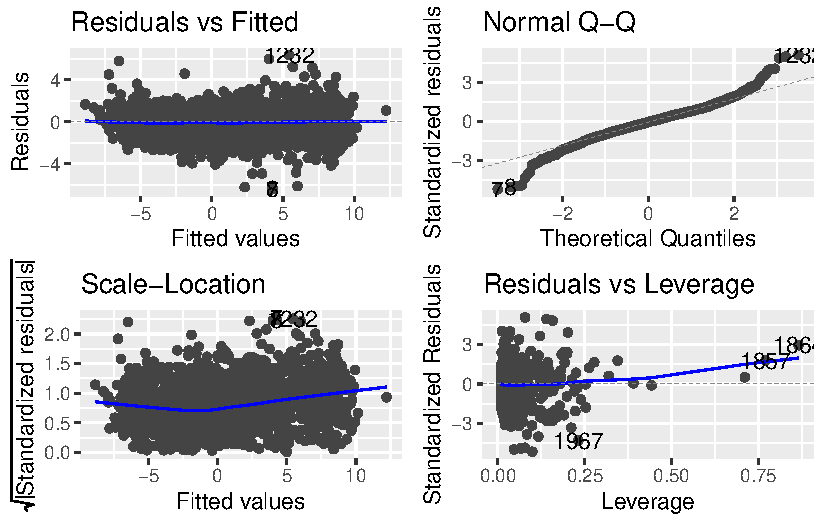
\includegraphics{seoul_files/figure-pdf/unnamed-chunk-14-2.pdf}

}

\end{figure}

\begin{verbatim}

Call:
lm(formula = TemperatureChange ~ 0 + ., data = seoul.subset[c("TemperatureChange", 
    elastic.factors)])

Residuals:
    Min      1Q  Median      3Q     Max 
-2.9227 -0.3435  0.0344  0.3820  3.9663 

Coefficients: (1 not defined because of singularities)
                                        Estimate Std. Error t value Pr(>|t|)
HumidityChange                        -2.173e-01  3.157e-03 -68.822  < 2e-16
DewPointTempChange                     7.373e-01  1.564e-02  47.150  < 2e-16
VisibilityChange                      -3.621e-04  4.325e-05  -8.372  < 2e-16
SolarRadiationChange                   6.018e-01  3.802e-02  15.831  < 2e-16
RainfallChange                         2.505e-02  8.708e-03   2.876 0.004065
Hour4Change                           -3.170e-01  7.280e-02  -4.354 1.40e-05
Hour5Change                           -1.370e-02  8.385e-02  -0.163 0.870194
Hour6Change                           -1.773e-01  9.400e-02  -1.886 0.059436
Hour8Change                           -2.363e-01  1.217e-01  -1.942 0.052220
Hour9Change                           -6.536e-01  1.320e-01  -4.951 7.97e-07
Hour10Change                          -5.119e-01  1.619e-01  -3.162 0.001588
Hour11Change                          -5.659e-01  1.436e-01  -3.941 8.37e-05
Hour12Change                          -5.208e-01  1.529e-01  -3.406 0.000671
Hour14Change                           2.690e-01  1.159e-01   2.320 0.020408
Hour15Change                           5.805e-01  1.542e-01   3.764 0.000172
Hour16Change                           2.904e-01  1.443e-01   2.012 0.044379
Hour17Change                           2.173e-02  1.426e-01   0.152 0.878932
Hour18Change                           2.911e-01  1.199e-01   2.427 0.015297
Hour19Change                           6.484e-01  8.365e-02   7.751 1.40e-14
Hour20Change                           4.540e-01  1.273e-01   3.567 0.000369
Hour21Change                           2.339e-01  9.997e-02   2.340 0.019386
HumidityChangeXDewPointTempChange     -3.178e-03  7.946e-04  -3.999 6.57e-05
DewPointTempChangeXVisibilityChange   -1.290e-04  2.506e-05  -5.149 2.87e-07
WindSpeedChangeXRainfallChange        -6.793e-03  6.172e-03  -1.101 0.271179
VisibilityChangeXSolarRadiationChange -4.926e-05  4.642e-05  -1.061 0.288734
SolarRadiationChangeXRainfallChange    8.332e-02  1.877e-02   4.439 9.49e-06
HumidityChangeXHour1Change            -1.083e-02  9.140e-03  -1.185 0.236216
HumidityChangeXHour2Change            -1.962e-02  7.941e-03  -2.471 0.013552
HumidityChangeXHour3Change            -3.413e-02  6.429e-03  -5.309 1.22e-07
HumidityChangeXHour5Change            -4.546e-02  9.115e-03  -4.987 6.62e-07
HumidityChangeXHour9Change             2.372e-03  8.897e-03   0.267 0.789786
HumidityChangeXHour10Change            1.549e-02  8.514e-03   1.820 0.068915
HumidityChangeXHour16Change           -3.080e-02  8.497e-03  -3.625 0.000295
HumidityChangeXHour17Change           -4.223e-02  8.207e-03  -5.145 2.92e-07
DewPointTempChangeXHour5Change         4.140e-01  5.194e-02   7.972 2.52e-15
DewPointTempChangeXHour6Change         1.420e-01  5.628e-02   2.522 0.011728
DewPointTempChangeXHour9Change         1.429e-01  5.812e-02   2.459 0.014009
DewPointTempChangeXHour11Change        1.058e-01  4.883e-02   2.167 0.030364
DewPointTempChangeXHour12Change        5.766e-02  3.905e-02   1.477 0.139956
DewPointTempChangeXHour13Change       -3.104e-02  4.168e-02  -0.745 0.456547
DewPointTempChangeXHour15Change       -1.879e-01  4.474e-02  -4.199 2.79e-05
DewPointTempChangeXHour18Change       -6.327e-02  3.792e-02  -1.669 0.095342
DewPointTempChangeXHour20Change       -1.487e-01  4.380e-02  -3.394 0.000701
DewPointTempChangeXHour21Change       -1.229e-01  3.978e-02  -3.090 0.002028
DewPointTempChangeXHour22Change       -1.315e-01  3.875e-02  -3.393 0.000704
WindSpeedChangeXHour5Change           -1.942e-02  7.484e-02  -0.259 0.795310
WindSpeedChangeXHour10Change          -6.487e-02  7.546e-02  -0.860 0.390103
WindSpeedChangeXHour14Change           8.693e-03  5.995e-02   0.145 0.884730
WindSpeedChangeXHour16Change           4.099e-02  5.685e-02   0.721 0.470983
WindSpeedChangeXHour19Change          -2.961e-02  6.366e-02  -0.465 0.641832
WindSpeedChangeXHour20Change          -6.298e-02  6.095e-02  -1.033 0.301534
VisibilityChangeXHour6Change           3.433e-04  1.715e-04   2.002 0.045431
VisibilityChangeXHour11Change          2.350e-06  1.804e-04   0.013 0.989607
VisibilityChangeXHour12Change          6.113e-05  1.626e-04   0.376 0.706936
VisibilityChangeXHour13Change         -5.348e-05  1.729e-04  -0.309 0.757156
VisibilityChangeXHour17Change          1.953e-04  1.794e-04   1.089 0.276441
VisibilityChangeXHour18Change          2.527e-04  1.633e-04   1.547 0.121903
SolarRadiationChangeXHour1Change      -3.891e-01  1.801e+00  -0.216 0.828933
SolarRadiationChangeXHour2Change       7.366e-01  3.725e-01   1.978 0.048107
SolarRadiationChangeXHour7Change      -8.378e-01  2.166e-01  -3.867 0.000113
SolarRadiationChangeXHour8Change      -7.240e-02  1.980e-01  -0.366 0.714663
SolarRadiationChangeXHour10Change      5.642e-01  9.858e-02   5.723 1.19e-08
SolarRadiationChangeXHour11Change      1.509e-01  5.844e-02   2.582 0.009890
SolarRadiationChangeXHour12Change     -4.064e-01  1.590e-01  -2.556 0.010658
SolarRadiationChangeXHour13Change      2.435e-01  1.761e-01   1.383 0.166915
SolarRadiationChangeXHour16Change     -3.989e-01  8.388e-02  -4.756 2.10e-06
SolarRadiationChangeXHour17Change     -9.066e-01  1.336e-01  -6.785 1.49e-11
SolarRadiationChangeXHour18Change     -7.024e-02  2.077e-01  -0.338 0.735270
SolarRadiationChangeXHour22Change             NA         NA      NA       NA
SolarRadiationChangeXHour23Change      5.892e-01  2.503e-01   2.354 0.018638
RainfallChangeXHour5Change            -3.724e-02  4.771e-02  -0.780 0.435208
RainfallChangeXHour20Change            4.282e-02  1.522e-02   2.813 0.004952
RainfallChangeXHour23Change           -4.084e-02  2.591e-02  -1.576 0.115099
                                         
HumidityChange                        ***
DewPointTempChange                    ***
VisibilityChange                      ***
SolarRadiationChange                  ***
RainfallChange                        ** 
Hour4Change                           ***
Hour5Change                              
Hour6Change                           .  
Hour8Change                           .  
Hour9Change                           ***
Hour10Change                          ** 
Hour11Change                          ***
Hour12Change                          ***
Hour14Change                          *  
Hour15Change                          ***
Hour16Change                          *  
Hour17Change                             
Hour18Change                          *  
Hour19Change                          ***
Hour20Change                          ***
Hour21Change                          *  
HumidityChangeXDewPointTempChange     ***
DewPointTempChangeXVisibilityChange   ***
WindSpeedChangeXRainfallChange           
VisibilityChangeXSolarRadiationChange    
SolarRadiationChangeXRainfallChange   ***
HumidityChangeXHour1Change               
HumidityChangeXHour2Change            *  
HumidityChangeXHour3Change            ***
HumidityChangeXHour5Change            ***
HumidityChangeXHour9Change               
HumidityChangeXHour10Change           .  
HumidityChangeXHour16Change           ***
HumidityChangeXHour17Change           ***
DewPointTempChangeXHour5Change        ***
DewPointTempChangeXHour6Change        *  
DewPointTempChangeXHour9Change        *  
DewPointTempChangeXHour11Change       *  
DewPointTempChangeXHour12Change          
DewPointTempChangeXHour13Change          
DewPointTempChangeXHour15Change       ***
DewPointTempChangeXHour18Change       .  
DewPointTempChangeXHour20Change       ***
DewPointTempChangeXHour21Change       ** 
DewPointTempChangeXHour22Change       ***
WindSpeedChangeXHour5Change              
WindSpeedChangeXHour10Change             
WindSpeedChangeXHour14Change             
WindSpeedChangeXHour16Change             
WindSpeedChangeXHour19Change             
WindSpeedChangeXHour20Change             
VisibilityChangeXHour6Change          *  
VisibilityChangeXHour11Change            
VisibilityChangeXHour12Change            
VisibilityChangeXHour13Change            
VisibilityChangeXHour17Change            
VisibilityChangeXHour18Change            
SolarRadiationChangeXHour1Change         
SolarRadiationChangeXHour2Change      *  
SolarRadiationChangeXHour7Change      ***
SolarRadiationChangeXHour8Change         
SolarRadiationChangeXHour10Change     ***
SolarRadiationChangeXHour11Change     ** 
SolarRadiationChangeXHour12Change     *  
SolarRadiationChangeXHour13Change        
SolarRadiationChangeXHour16Change     ***
SolarRadiationChangeXHour17Change     ***
SolarRadiationChangeXHour18Change        
SolarRadiationChangeXHour22Change        
SolarRadiationChangeXHour23Change     *  
RainfallChangeXHour5Change               
RainfallChangeXHour20Change           ** 
RainfallChangeXHour23Change              
---
Signif. codes:  0 '***' 0.001 '**' 0.01 '*' 0.05 '.' 0.1 ' ' 1

Residual standard error: 0.7192 on 2131 degrees of freedom
Multiple R-squared:  0.9621,    Adjusted R-squared:  0.9608 
F-statistic: 751.8 on 72 and 2131 DF,  p-value: < 2.2e-16
\end{verbatim}

\begin{figure}[H]

{\centering 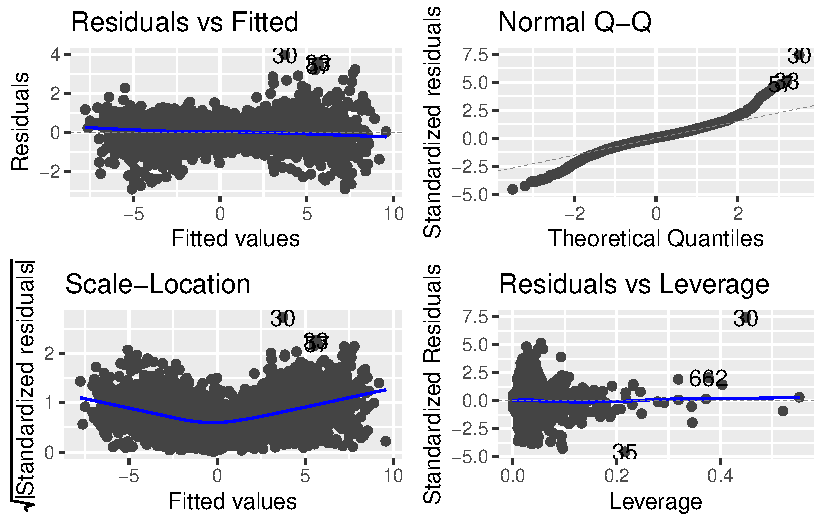
\includegraphics{seoul_files/figure-pdf/unnamed-chunk-14-3.pdf}

}

\end{figure}

\begin{verbatim}

Call:
lm(formula = TemperatureChange ~ 0 + ., data = seoul.subset[c("TemperatureChange", 
    elastic.factors)])

Residuals:
    Min      1Q  Median      3Q     Max 
-6.1285 -0.4940 -0.0988  0.3265  5.5903 

Coefficients:
                                          Estimate Std. Error t value Pr(>|t|)
HumidityChange                          -2.144e-01  2.894e-03 -74.097  < 2e-16
DewPointTempChange                       7.525e-01  1.207e-02  62.356  < 2e-16
WindSpeedChange                          7.905e-03  2.016e-02   0.392 0.694974
VisibilityChange                        -3.982e-04  5.732e-05  -6.948 4.92e-12
SolarRadiationChange                     5.719e-01  4.075e-02  14.035  < 2e-16
RainfallChange                           4.997e-02  1.522e-02   3.282 0.001046
Hour5Change                             -1.092e-01  8.384e-02  -1.303 0.192783
Hour14Change                             7.987e-01  1.160e-01   6.886 7.50e-12
Hour15Change                             1.293e+00  1.088e-01  11.886  < 2e-16
Hour16Change                             8.967e-01  1.261e-01   7.112 1.55e-12
Hour17Change                             5.262e-01  1.044e-01   5.040 5.05e-07
Hour18Change                             3.929e-01  1.171e-01   3.355 0.000806
Hour19Change                             5.959e-01  9.148e-02   6.514 9.11e-11
Hour20Change                             4.248e-01  9.096e-02   4.670 3.20e-06
Hour21Change                             3.242e-01  8.689e-02   3.732 0.000195
DewPointTempChangeXSolarRadiationChange  4.035e-02  8.889e-03   4.539 5.96e-06
VisibilityChangeXSolarRadiationChange   -1.757e-04  6.020e-05  -2.919 0.003554
SolarRadiationChangeXRainfallChange      1.500e-01  3.781e-02   3.966 7.54e-05
SolarRadiationChangeXSnowfallChange      6.025e-01  1.221e-01   4.936 8.61e-07
HumidityChangeXHour8Change               1.712e-02  5.679e-03   3.014 0.002606
HumidityChangeXHour9Change               5.218e-02  9.119e-03   5.722 1.20e-08
HumidityChangeXHour10Change              2.795e-02  1.002e-02   2.790 0.005322
HumidityChangeXHour14Change             -3.710e-03  6.718e-03  -0.552 0.580800
HumidityChangeXHour15Change             -1.221e-02  6.472e-03  -1.887 0.059283
HumidityChangeXHour16Change             -2.185e-02  6.566e-03  -3.329 0.000888
HumidityChangeXHour23Change             -8.744e-03  6.558e-03  -1.333 0.182571
DewPointTempChangeXHour4Change           9.340e-02  3.990e-02   2.341 0.019342
DewPointTempChangeXHour10Change          2.111e-02  3.919e-02   0.539 0.590216
DewPointTempChangeXHour11Change          3.105e-02  2.668e-02   1.164 0.244672
DewPointTempChangeXHour18Change         -1.316e-01  2.811e-02  -4.684 2.99e-06
DewPointTempChangeXHour19Change         -9.718e-02  2.952e-02  -3.292 0.001011
DewPointTempChangeXHour20Change         -1.183e-01  2.798e-02  -4.230 2.44e-05
DewPointTempChangeXHour21Change         -1.127e-01  2.804e-02  -4.020 6.01e-05
DewPointTempChangeXHour22Change         -5.369e-02  2.856e-02  -1.880 0.060259
WindSpeedChangeXHour14Change             2.529e-02  6.813e-02   0.371 0.710509
WindSpeedChangeXHour15Change             8.328e-02  5.959e-02   1.398 0.162387
VisibilityChangeXHour10Change            4.444e-05  1.614e-04   0.275 0.783047
VisibilityChangeXHour11Change           -1.585e-04  1.687e-04  -0.939 0.347771
VisibilityChangeXHour22Change            1.648e-04  2.140e-04   0.770 0.441429
SolarRadiationChangeXHour5Change        -1.465e-01  1.501e-01  -0.976 0.329364
SolarRadiationChangeXHour8Change        -5.757e-01  1.332e-01  -4.322 1.62e-05
SolarRadiationChangeXHour9Change        -5.358e-02  1.238e-01  -0.433 0.665286
SolarRadiationChangeXHour11Change        1.338e-01  6.010e-02   2.225 0.026160
SolarRadiationChangeXHour12Change        3.630e-01  4.991e-02   7.273 4.93e-13
SolarRadiationChangeXHour13Change        1.019e-02  8.146e-02   0.125 0.900502
SolarRadiationChangeXHour16Change       -6.820e-01  1.376e-01  -4.958 7.67e-07
SolarRadiationChangeXHour22Change        8.806e-01  2.008e-01   4.386 1.21e-05
SolarRadiationChangeXHour23Change        1.421e+00  4.376e-01   3.247 0.001183
RainfallChangeXHour9Change              -1.421e-01  5.962e-02  -2.384 0.017213
RainfallChangeXHour20Change             -2.360e-01  8.713e-02  -2.709 0.006797
                                           
HumidityChange                          ***
DewPointTempChange                      ***
WindSpeedChange                            
VisibilityChange                        ***
SolarRadiationChange                    ***
RainfallChange                          ** 
Hour5Change                                
Hour14Change                            ***
Hour15Change                            ***
Hour16Change                            ***
Hour17Change                            ***
Hour18Change                            ***
Hour19Change                            ***
Hour20Change                            ***
Hour21Change                            ***
DewPointTempChangeXSolarRadiationChange ***
VisibilityChangeXSolarRadiationChange   ** 
SolarRadiationChangeXRainfallChange     ***
SolarRadiationChangeXSnowfallChange     ***
HumidityChangeXHour8Change              ** 
HumidityChangeXHour9Change              ***
HumidityChangeXHour10Change             ** 
HumidityChangeXHour14Change                
HumidityChangeXHour15Change             .  
HumidityChangeXHour16Change             ***
HumidityChangeXHour23Change                
DewPointTempChangeXHour4Change          *  
DewPointTempChangeXHour10Change            
DewPointTempChangeXHour11Change            
DewPointTempChangeXHour18Change         ***
DewPointTempChangeXHour19Change         ** 
DewPointTempChangeXHour20Change         ***
DewPointTempChangeXHour21Change         ***
DewPointTempChangeXHour22Change         .  
WindSpeedChangeXHour14Change               
WindSpeedChangeXHour15Change               
VisibilityChangeXHour10Change              
VisibilityChangeXHour11Change              
VisibilityChangeXHour22Change              
SolarRadiationChangeXHour5Change           
SolarRadiationChangeXHour8Change        ***
SolarRadiationChangeXHour9Change           
SolarRadiationChangeXHour11Change       *  
SolarRadiationChangeXHour12Change       ***
SolarRadiationChangeXHour13Change          
SolarRadiationChangeXHour16Change       ***
SolarRadiationChangeXHour22Change       ***
SolarRadiationChangeXHour23Change       ** 
RainfallChangeXHour9Change              *  
RainfallChangeXHour20Change             ** 
---
Signif. codes:  0 '***' 0.001 '**' 0.01 '*' 0.05 '.' 0.1 ' ' 1

Residual standard error: 0.843 on 2129 degrees of freedom
Multiple R-squared:  0.9568,    Adjusted R-squared:  0.9558 
F-statistic: 943.3 on 50 and 2129 DF,  p-value: < 2.2e-16
\end{verbatim}

\begin{figure}[H]

{\centering 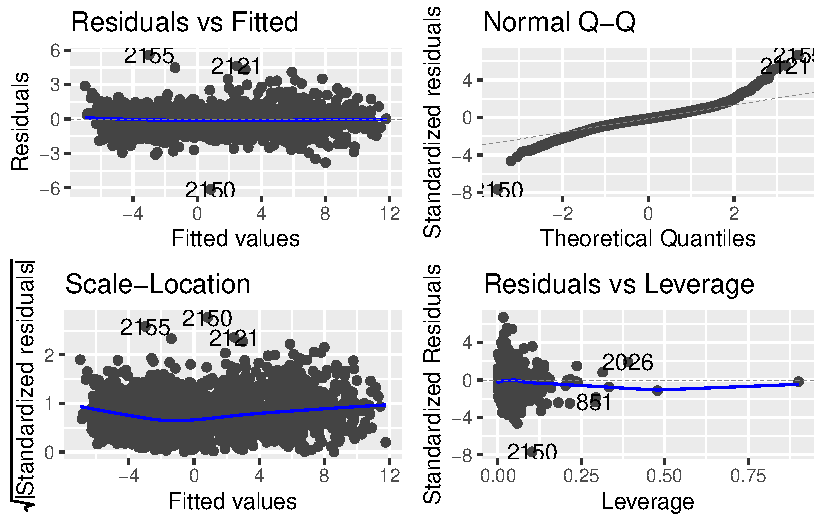
\includegraphics{seoul_files/figure-pdf/unnamed-chunk-14-4.pdf}

}

\end{figure}

\hypertarget{a5}{%
\paragraph{A.5}\label{a5}}

Most assailant factors in Model (2) (hour changes excluded)

\begin{Shaded}
\begin{Highlighting}[]
\NormalTok{elastic.coef }\OtherTok{=} \FunctionTok{tibble}\NormalTok{(}
  \AttributeTok{Factor =} \FunctionTok{names}\NormalTok{(seoul.elastic}\SpecialCharTok{$}\NormalTok{coefficients),}
  \AttributeTok{Coefficient =}\NormalTok{ seoul.elastic}\SpecialCharTok{$}\NormalTok{coefficients}
\NormalTok{)}

\NormalTok{elastic.coef }\SpecialCharTok{\%\textgreater{}\%} \FunctionTok{arrange}\NormalTok{(}\FunctionTok{abs}\NormalTok{(Coefficient) }\SpecialCharTok{\%\textgreater{}\%} \FunctionTok{desc}\NormalTok{()) }\SpecialCharTok{\%\textgreater{}\%} 
  \FunctionTok{filter}\NormalTok{(}\SpecialCharTok{!}\NormalTok{(Factor }\SpecialCharTok{\%in\%} \FunctionTok{str\_c}\NormalTok{(time.bike, }\StringTok{"Change"}\NormalTok{))) }\SpecialCharTok{\%\textgreater{}\%}
\NormalTok{  knitr}\SpecialCharTok{::}\FunctionTok{kable}\NormalTok{()}
\end{Highlighting}
\end{Shaded}

\begin{longtable}[]{@{}lr@{}}
\toprule\noalign{}
Factor & Coefficient \\
\midrule\noalign{}
\endhead
\bottomrule\noalign{}
\endlastfoot
SolarRadiationChangeXHour1Change & 5.9532135 \\
SolarRadiationChangeXHour4Change & -0.9430467 \\
SolarRadiationChange & 0.9373443 \\
SolarRadiationChangeXHour2Change & 0.8983334 \\
SolarRadiationChangeXHour11Change & 0.8079038 \\
SolarRadiationChangeXHour5Change & -0.5630207 \\
DewPointTempChange & 0.5567638 \\
SolarRadiationChangeXHour3Change & -0.5384046 \\
SolarRadiationChangeXHour23Change & 0.5273883 \\
SolarRadiationChangeXHour10Change & 0.5050862 \\
SolarRadiationChangeXHour12Change & 0.4593210 \\
SnowfallChangeXHour19Change & 0.4065894 \\
SolarRadiationChangeXHour13Change & 0.3968544 \\
SnowfallChange & 0.3596363 \\
SolarRadiationChangeXHour7Change & -0.3072783 \\
WindSpeedChangeXHour6Change & 0.2357548 \\
SnowfallChangeXHour10Change & -0.2215750 \\
SolarRadiationChangeXHour17Change & -0.2005535 \\
SnowfallChangeXHour8Change & -0.1881401 \\
DewPointTempChangeXHour1Change & 0.1850268 \\
DewPointTempChangeXHour10Change & -0.1671382 \\
SolarRadiationChangeXHour14Change & 0.1626236 \\
WindSpeedChangeXHour5Change & 0.1530196 \\
HumidityChange & -0.1527853 \\
DewPointTempChangeXHour19Change & -0.1357014 \\
RainfallChangeXHour10Change & -0.1236390 \\
SolarRadiationChangeXHour20Change & -0.1125570 \\
HumidityChangeXHour10Change & 0.1104926 \\
DewPointTempChangeXHour2Change & 0.1104755 \\
DewPointTempChangeXHour11Change & -0.1079877 \\
SolarRadiationChangeXRainfallChange & 0.1030836 \\
WindSpeedChangeXHour4Change & 0.0936037 \\
RainfallChangeXHour9Change & -0.0806904 \\
WindSpeedChangeXHour3Change & 0.0784248 \\
SnowfallChangeXHour9Change & -0.0772055 \\
WindSpeedChangeXHour17Change & -0.0751434 \\
RainfallChangeXHour14Change & 0.0707324 \\
DewPointTempChangeXHour18Change & -0.0694302 \\
HumidityChangeXHour11Change & 0.0676864 \\
HumidityChangeXHour9Change & 0.0667211 \\
WindSpeedChangeXHour19Change & -0.0654506 \\
DewPointTempChangeXHour20Change & 0.0599091 \\
RainfallChangeXHour20Change & 0.0553282 \\
HumidityChangeXHour5Change & 0.0531223 \\
WindSpeedChange & 0.0513840 \\
HumidityChangeXHour19Change & 0.0491966 \\
WindSpeedChangeXHour18Change & -0.0464846 \\
HumidityChangeXHour6Change & 0.0433121 \\
HumidityChangeXHour8Change & 0.0432974 \\
HumidityChangeXHour2Change & -0.0398986 \\
HumidityChangeXHour1Change & -0.0393130 \\
RainfallChangeXHour21Change & 0.0372447 \\
WindSpeedChangeXSolarRadiationChange & 0.0364910 \\
HumidityChangeXHour23Change & -0.0362853 \\
DewPointTempChangeXHour21Change & -0.0294300 \\
HumidityChangeXHour14Change & 0.0261822 \\
HumidityChangeXHour12Change & 0.0244775 \\
HumidityChangeXHour15Change & 0.0244668 \\
HumidityChangeXHour7Change & 0.0237191 \\
HumidityChangeXHour22Change & -0.0224267 \\
WindSpeedChangeXHour11Change & 0.0217454 \\
DewPointTempChangeXWindSpeedChange & 0.0205411 \\
HumidityChangeXSolarRadiationChange & 0.0136437 \\
HumidityChangeXHour4Change & 0.0130725 \\
DewPointTempChangeXHour13Change & -0.0115377 \\
DewPointTempChangeXHour14Change & -0.0093712 \\
HumidityChangeXHour16Change & 0.0049636 \\
DewPointTempChangeXRainfallChange & -0.0040924 \\
HumidityChangeXHour17Change & -0.0035436 \\
HumidityChangeXSnowfallChange & -0.0031202 \\
HumidityChangeXRainfallChange & -0.0022643 \\
DewPointTempChangeXHour4Change & -0.0020395 \\
WindSpeedChangeXHour10Change & -0.0017256 \\
HumidityChangeXDewPointTempChange & -0.0012633 \\
VisibilityChangeXHour23Change & -0.0006304 \\
VisibilityChangeXHour2Change & -0.0004989 \\
VisibilityChangeXHour1Change & -0.0003839 \\
VisibilityChange & -0.0003557 \\
VisibilityChangeXHour8Change & 0.0003071 \\
VisibilityChangeXHour19Change & 0.0003042 \\
VisibilityChangeXHour4Change & -0.0002668 \\
VisibilityChangeXHour16Change & 0.0001461 \\
VisibilityChangeXHour9Change & 0.0001102 \\
VisibilityChangeXHour3Change & -0.0000825 \\
VisibilityChangeXHour17Change & 0.0000804 \\
WindSpeedChangeXVisibilityChange & 0.0000758 \\
VisibilityChangeXHour20Change & -0.0000294 \\
VisibilityChangeXHour11Change & -0.0000131 \\
WindSpeedChangeXHour15Change & 0.0000089 \\
\end{longtable}

\hypertarget{a6}{%
\paragraph{A.6}\label{a6}}

The theoretical model for Model (2) can be fully written as,

\begin{enumerate}
\def\labelenumi{(\arabic{enumi})}
\setcounter{enumi}{1}
\tightlist
\item
  \(\Delta\text{Temperature}_{st} = \beta_1\Delta\text{Humidity}_{st} + \beta_2\Delta\text{DewPointTemp}_{st} + \beta_3\Delta\text{Visibility}_{st} + \beta_4\Delta\text{WindSpeed}_{st} + \beta_5\Delta\text{SolarRadiation}_{st} + \beta_6\Delta\text{Rainfall}_{st} + \beta_7\Delta\text{Snowfall}_{st} + \beta_8\Delta I(\text{Hour}_{t} = 1) + ... + \beta_{30}\Delta I(\text{Hour}_{t} = 23) + \beta_{31}\Delta\text{Humidity}_{st}\text{DewPointTemp}_{st} + \beta_{32}\Delta\text{Humidity}_{st}\text{SolarRadiation}_{st}+\beta_{33}\Delta\text{Humidity}_{st}\text{Rainfall}_{st} + \beta_{34}\Delta\text{Humidity}_{st}\text{Snowfall}_{st} + \beta_{35}\Delta\text{DewPointTemp}_{st}\text{WindSpeed}_{st} + \beta_{36}\Delta\text{DewPointTemp}_{st}\text{Rainfall}_{st} + \beta_{37}\Delta\text{WindSpeed}_{st}\text{Visibility}_{st}+\beta_{38}\Delta\text{WindSpeed}_{st}\text{solarRadiation}_{st} + \beta_{39}\Delta\text{SolarRadiation}_{st}\text{Rainfall}_{st}+ \\ \sum_{j=1}^{23}{\beta_{39+j}\Delta\text{Humidity}_{st}\Delta I(\text{Hour}_t=j)}+\sum_{k=1}^{23}{\beta_{62+k}\Delta\text{DewPointTemp}_{st}\Delta I(\text{Hour}_t=k)}+\sum_{l=1}^{23}{\beta_{85+l}\Delta\text{WindSpeed}_{st}\Delta I(\text{Hour}_t=l)}+\sum_{m=1}^{23}{\beta_{108+m}\Delta\text{Visibility}_{st}\Delta I(\text{Hour}_t=m)}+\sum_{n=1}^{23}{\beta_{131+n}\Delta\text{SolarRadiation}_{st}\Delta I(\text{Hour}_t=n)}+\sum_{o=1}^{23}{\beta_{154+o}\Delta\text{Rainfall}_{st}\Delta I(\text{Hour}_t=o)}+\sum_{p=1}^{23}{\beta_{177+p}\Delta\text{Snowfall}_{st}\Delta I(\text{Hour}_t=p)} + \Delta\eta_{st}\)
\end{enumerate}

\(\Delta\eta_{st} \overset{iid}{\sim} N(0, \sigma^2)\)

Due to the nature of elastic net regression, some of the coefficients
for \(j, k, l, m, n, o,\) and \(p\) are \(0\):

\(\beta_{39+j} = 0 \quad \forall j \in \{3,13,15,18,20\}\)

\(\beta_{62+k} = 0 \quad \forall k \in \{3,5,6,7,8,12,15,22,23\}\)

\(\beta_{85+l} = 0 \quad \forall l \in \{1,2,3,7,8,9,12,13,14,16,20,21,22,23\}\)

\(\beta_{108+m} = 0 \quad \forall m \in \{5,6,7,,10,12,13,14,15,18,21,22\}\)

\(\beta_{131+n} = 0 \quad \forall n \in \{8,9,15,16,18,21,22\}\)

\(\beta_{154+o} = 0 \quad \forall o \in \{1,...,8,11,12,13,15,16,17,18,19,23\}\)

\(\beta_{177+p} = 0 \quad \forall p \in \{1,...,7,11,...,15,17,18,20,21,22,23\}\)



\end{document}
